\documentclass[11pt]{article}
 
\newcommand\CG[1]{\textcolor{red}{#1}}

\usepackage{lineno,hyperref}

\usepackage[margin=1 in]{geometry}
\renewcommand{\baselinestretch}{1.25}


%\usepackage{refcheck}
\usepackage{authblk}
\usepackage{galois} % composition function \comp
\usepackage{bm}
\usepackage{amsmath}
\usepackage{amssymb}
\usepackage{mathrsfs}
\usepackage{amsthm}
\usepackage{natbib}
\usepackage{graphicx}
\usepackage{color}
\usepackage{booktabs}
\usepackage[page,title]{appendix}
%\renewcommand\appendixname{haha}
\usepackage{enumerate}
\usepackage{changepage}
\usepackage{datetime}
\usepackage[FIGTOPCAP]{subfigure}
\newdate{date}{9}{1}{2017}

%%%%%%%%%%%%%%  Notations %%%%%%%%%%
\DeclareMathOperator{\mytr}{tr}
\DeclareMathOperator{\mydiag}{diag}
\DeclareMathOperator{\myRank}{Rank}
\DeclareMathOperator{\myP}{P}
\DeclareMathOperator{\myE}{E}
\DeclareMathOperator{\myVar}{Var}
\DeclareMathOperator{\myCov}{Cov}
\DeclareMathOperator*{\argmax}{arg\,max}
\DeclareMathOperator*{\argmin}{arg\,min}


\newcommand{\Ba}{\mathbf{a}}    \newcommand{\Bb}{\mathbf{b}}    \newcommand{\Bc}{\mathbf{c}}    \newcommand{\Bd}{\mathbf{d}}    \newcommand{\Be}{\mathbf{e}}    \newcommand{\Bf}{\mathbf{f}}    \newcommand{\Bg}{\mathbf{g}}    \newcommand{\Bh}{\mathbf{h}}    \newcommand{\Bi}{\mathbf{i}}    \newcommand{\Bj}{\mathbf{j}}    \newcommand{\Bk}{\mathbf{k}}    \newcommand{\Bl}{\mathbf{l}}
\newcommand{\Bm}{\mathbf{m}}    \newcommand{\Bn}{\mathbf{n}}    \newcommand{\Bo}{\mathbf{o}}    \newcommand{\Bp}{\mathbf{p}}    \newcommand{\Bq}{\mathbf{q}}    \newcommand{\Br}{\mathbf{r}}    \newcommand{\Bs}{\mathbf{s}}    \newcommand{\Bt}{\mathbf{t}}    \newcommand{\Bu}{\mathbf{u}}    \newcommand{\Bv}{\mathbf{v}}    \newcommand{\Bw}{\mathbf{w}}    \newcommand{\Bx}{\mathbf{x}}
\newcommand{\By}{\mathbf{y}}    \newcommand{\Bz}{\mathbf{z}}    
\newcommand{\BA}{\mathbf{A}}    \newcommand{\BB}{\mathbf{B}}    \newcommand{\BC}{\mathbf{C}}    \newcommand{\BD}{\mathbf{D}}    \newcommand{\BE}{\mathbf{E}}    \newcommand{\BF}{\mathbf{F}}    \newcommand{\BG}{\mathbf{G}}    \newcommand{\BH}{\mathbf{H}}    \newcommand{\BI}{\mathbf{I}}    \newcommand{\BJ}{\mathbf{J}}    \newcommand{\BK}{\mathbf{K}}    \newcommand{\BL}{\mathbf{L}}
\newcommand{\BM}{\mathbf{M}}    \newcommand{\BN}{\mathbf{N}}    \newcommand{\BO}{\mathbf{O}}    \newcommand{\BP}{\mathbf{P}}    \newcommand{\BQ}{\mathbf{Q}}    \newcommand{\BR}{\mathbf{R}}    \newcommand{\BS}{\mathbf{S}}    \newcommand{\BT}{\mathbf{T}}    \newcommand{\BU}{\mathbf{U}}    \newcommand{\BV}{\mathbf{V}}    \newcommand{\BW}{\mathbf{W}}    \newcommand{\BX}{\mathbf{X}}
\newcommand{\BY}{\mathbf{Y}}    \newcommand{\BZ}{\mathbf{Z}}    

\newcommand{\bfsym}[1]{\ensuremath{\boldsymbol{#1}}}

 \def\balpha{\bfsym \alpha}
 \def\bbeta{\bfsym \beta}
 \def\bgamma{\bfsym \gamma}             \def\bGamma{\bfsym \Gamma}
 \def\bdelta{\bfsym {\delta}}           \def\bDelta {\bfsym {\Delta}}
 \def\bfeta{\bfsym {\eta}}              \def\bfEta {\bfsym {\Eta}}
 \def\bmu{\bfsym {\mu}}                 \def\bMu {\bfsym {\Mu}}
 \def\bnu{\bfsym {\nu}}
 \def\btheta{\bfsym {\theta}}           \def\bTheta {\bfsym {\Theta}}
 \def\beps{\bfsym \varepsilon}          \def\bepsilon{\bfsym \epsilon}
 \def\bsigma{\bfsym \sigma}             \def\bSigma{\bfsym \Sigma}
 \def\blambda {\bfsym {\lambda}}        \def\bLambda {\bfsym {\Lambda}}
 \def\bomega {\bfsym {\omega}}          \def\bOmega {\bfsym {\Omega}}
 \def\brho   {\bfsym {\rho}}
 \def\btau{\bfsym {\tau}}
 \def\bxi{\bfsym {\xi}}
 \def\bzeta{\bfsym {\zeta}}
% May add more in future.
%%%%%%%%%%%%%%%%%%%%%%%%%%%%%%%%%%%%



\theoremstyle{plain}
\newtheorem{theorem}{\quad\quad Theorem}
\newtheorem{proposition}{\quad\quad Proposition}
\newtheorem{corollary}{\quad\quad Corollary}
\newtheorem{lemma}{\quad\quad Lemma}
\newtheorem{example}{Example}
\newtheorem{assumption}{\quad\quad Assumption}
\newtheorem{condition}{\quad\quad Condition}

\theoremstyle{definition}
\newtheorem{definition}{\quad\quad Definition}
\newtheorem{remark}{\quad\quad Remark}
\theoremstyle{remark}





\begin{document}
\title{
A Bayesian-motivated test for high-dimensional linear model with fixed design
}



\author[1]{Rui Wang}
\author[1,2]{Xingzhong Xu\thanks{Corresponding author\\Email address: xuxz@bit.edu.cn}}
\affil[1]{
School of Mathematics and Statistics, Beijing Institute of Technology, Beijing 
    100081,China
}
\affil[2]{
Beijing Key Laboratory on MCAACI, Beijing Institute of Technology, Beijing 100081,China
}

\maketitle
\begin{abstract}
    This paper considers testing regression coefficients in high-dimensional linear model with fixed design matrix.
    We prove that there does not exist nontrivial unbiased test for this problem.
    This phenomenon makes it impossible to consider the problem from a minimax perspective.
    We propose a new test statistic which is the limit of Bayes factors under normal distribution.
    The null distribution of the test statistic is approximated by Lindeberg's replacement trick.
    Under certain conditions, we also give the global asymptotic power function of the proposed test.
    It turns out that the proposed test has good power behavior when the signal is strong.
    The performance of the proposed test is examined by simulation results.

\end{abstract}

\noindent {\it Key words}: High-dimensional test, Lindeberg method, Linear model, Unbiasedness.

\section{Introduction} 
Consider linear regression model of the form
\begin{equation}\label{label:linearModel}
    \By = 
    \BX_a \bbeta_a + \BX_b \bbeta_b + \bepsilon, %\quad \bepsilon\sim \mathcal N_n(0,\phi^{-1} \BI_n),
\end{equation}
where $\By \in \mathbb R^n$ is the response, $\BX_a$, $\BX_b$ are $n\times q$ and $n\times p$ design matrices, respectively,  $\bbeta_a\in \mathbb R^q$, $\bbeta_b\in \mathbb R^p$ are unknown regression coefficients, and 
$\bepsilon\in \mathbb R^n$ is the vector of random errors.
Here the design matrix $\BX_a$ contains the predictors that are known to have effects on the response,
and our interest is to test if $\BX_b$ contains any useful predictors.
That is, we would like to test the hypotheses
\begin{align}\label{theHypothesis}
    \mathcal H_0:   \bbeta_b =0,\quad
    \text{v.s.} \quad
    \mathcal H_1:   \bbeta_b \neq 0.
\end{align}
%Motivated by many recent applications of high dimensional regression, we consider the situation where $p+q$ is much larger than $n$.
The conventional test for hypotheses \eqref{theHypothesis} is the $F$-test which is also the likelihood ratio test under normal errors.
However, the $F$-test is not well defined in high dimensional setting.
In fact, if $\bepsilon$ is normal distributed and $\myRank[\BX_a;\BX_b]=n$, then the likelihood is unbounded under the alternative hypothesis.
Thus, new test methodology is required in high-dimensional setting.

For the problem of testing hypotheses\eqref{theHypothesis}, two different high-dimensional settings have been extensively considered in the literature.
One is the small $p$, large $q$ setting.
An important example of this setting is testing individual coefficients of a high-dimensional regression.
See \cite{buhlmann2013statistical}, \cite{Zhang2013} and \cite{Lan2016} for testing procedures in this setting.
In this paper, however, we focus on the other setting, namely the large $p$, small $q$ setting.
In this case, there are just a few covariates, namely $\BX_a$, are known to have effects on the response, while there remain a large number of covariates, namely $\BX_b$, to be tested.
%We assume $\BX_a$ has full column rank and $\BX_b$ has full row rank.
%In practice, which covariates belong to the part $\BX_a$ is determined apriori.
%If no prior knowledge is available, $\BX_a$ can be $\mathbf 1_n$.
%In both cases, $q$ is often relatively small.
%However, there may remain a very large number of variables in $\BX_b$, so $p>n$.

Many test procedures have been proposed in the large $p$, small $q$ setting.
Based on an empirical Bayes model, \cite{Goeman2006} and \cite{Goeman2011} proposed a score test statistic as well as a method to determine the critical value.
This score test was further investigated by \cite{Lan2014Testing} and \cite{Lan2016a}.
Based on $U$-statistics, \cite{Zhong2011Tests} proposed a test for the case where $\BX_a=\mathbf 1_n$.
Later, \cite{Wang2015} extended the test of \cite{Zhong2011Tests} to the case where $\BX_a$ is a general design matrix.
To accommodate outlying observations and heavy-tailed distributions, \cite{Feng2013}
proposed a rank-based test for the entire coefficients.
\cite{Xu2016a} modified \cite{Feng2013}'s test and proposed a scalar invariant rank-based test.
\cite{Janson2016} utilized a convex optimization program to obtain an unbiased estimator of a signal to noise ratio with small variance, based on which a test is constructed.
Apart from the afore mentioned tests,
there is another line of research utilizing desparsified Lasso estimator; see \cite{Dezeure2017} and the references therein.

Except for the test of \cite{Goeman2006}, most existing high dimensional tests adopted the random design assumption, that is, the rows of $\BX_b$ are considered as being generated from a super population.
As noted by \cite{Lei2018}, assuming a fixed design or a random design could lead to qualitatively different inferential results and the former is preferable from a theoretical point of view.
Hence we focus on the fixed design setting in this paper.
Of course, our results are still valid for random design from a conditional inference perspective.




In Bayesian literature, many Bayesian tests have been proposed for hypothesis \eqref{theHypothesis} in low-dimensional setting; see \cite{javier2006Obj,Goddard2016,zhou2018On} and the references therein.
So far, most existing Bayesian tests are not applicable in large $p$, small $q$ setting.
In principle,
using Bayes factor as a frequentist test statistic in high-dimensional setting is a good strategy for at least two reasons.
First, the Bayes factors corresponding to proper priors are always well defined, even if the likelihood is unbounded.
Second, under mild conditions, tests based on Bayes factors are admissible (See, e.g., \cite{Lehmann}, Theorem 6.7.2).
In fact, the test procedure of \cite{Goeman2006} is motivated by Bayesian methods but is treated as a frequentist significance test.


In this paper, we propose a new test statistic in large $p$, small $q$ setting which is the limit of Bayes factors under normal linear model.
The proposed test statistic is a ratio of quadratic forms of $\By$.
We give an approximation of the distribution of quadratic form using Lindeberg's replacement trick.
Based on this approximated distribution, the critical value of the proposed test statisitc is calculated by a one step iteration.
We prove that the proposed test procedure is valid under weak conditions.
In particular, we do not require that the test statistic is asymptotically normally distributed.
Under certain conditions, we also derive the asymptotic power function of the proposed test and the test of \cite{Goeman2006}.
A simulation is conducted to examine the performance of the proposed test.
It turns out that the proposed test is powerful especially when $\|\bbeta_b\|$ is large.

The rest of the paper is organized as follows.
In Section \ref{sec:methodology}, we propose a Bayesian-motivated test and study the theoretical properties of the proposed test procedure.
The asymptotic power function is also derived.
Section \ref{sec:Numerical} contains the simulation results. 
Section \ref{sec:conclusions} concludes the paper.
The technical proofs are presented in Appendix.




\section{Test procedure}\label{sec:methodology}
\subsection{A Bayesian-motivated test}
In this paper, we consider testing hypotheses \eqref{theHypothesis} in large $p$, small $q$ setting.
More specifically, we make the following assumption throughout the paper.
\begin{assumption}
    In the linear model \eqref{label:linearModel}, 
    suppose $\bepsilon=(\epsilon_1,\ldots,\epsilon_n)^\top$ where $\epsilon_1,\ldots, \epsilon_n$ are independent indentically distributed (iid) with mean $0$ and covariance $\sigma^2=\phi^{-1}$.
    Furthermore, suppose $q<n$, $\myRank(\BX_a)=q$ and $\myRank([\BX_a; \BX_b])=n$.
    \label{Assumption}
\end{assumption}
%Based on an empirical Bayes model,
%\cite{Goeman2006} and \cite{Goeman2011} proposed a score test which can be used.
Testing hypotheses \eqref{theHypothesis} in large $p$, small $q$ setting is a challenging problem.
\cite{Goeman2006} noticed that their test has negligible power for many alternatives and consequently is not an unbiased test.
Biased tests are often regarded as problematic in classical statistics.
However, the situation is very different for our problem.
In fact, we shall show that under normal assumption, there is no nontrivial unbiased test in large $p$, small $q$ setting.

Let $\BP_a=\BX_a(\BX_a^\top \BX_a)^{-1} \BX^\top$ be the projection matrix onto the column space of $\BX_a$ and denote $\tilde \BP_a = \BI_n-\BP_a$.
Define $\btheta =(\bbeta_a^\top , \bbeta_b^\top , \phi)^\top$ and 
\begin{equation*}
    \begin{split}
        &\Theta_0 = \left\{\theta=(\bbeta_a^\top , \bbeta_b^\top , \phi)^\top: \bbeta_a \in \mathbb R^{q}, \bbeta_b=0, \phi>0\right\},
    \\
    &\Theta = \left\{\theta=(\bbeta_a^\top , \bbeta_b^\top , \phi)^\top: \bbeta_a \in \mathbb R^{q}, \bbeta_b\in \mathbb R^p, \phi>0\right\}.
    \end{split}
\end{equation*}
A test function $\varphi(\By)$ of level $\alpha$ is a Borel measurable function from $\mathbb R^n$ to $\mathbb R$ such that $0\leq \varphi(\By) \leq 1$ and $\myE_\theta [\varphi(\By)]\leq \alpha$ for $\theta\in \Theta_0$.
A test function $\varphi(\By)$ is nonrandom if $\varphi(\By)\in\{0,1\}$.
Let $\lambda(\cdot)$ be the Lebesgue measure on $\mathbb R^n$.
We have the following proposition.
\begin{proposition}\label{prop:unbiased}
    Suppose Assumption \ref{Assumption} holds.
    Furthermore, assume $\bepsilon\sim \mathcal N_n (0, \phi^{-1}\BI_n)$.
    Let $\varphi(\By)$ be a test function of level $\alpha$, $0 <\alpha <1$.
Then the following results hold.
\begin{enumerate}[(a)]
    \item 
        If $\varphi(\By)$ is unbiased, that is, $\myE_\theta [\varphi(\By)]\geq \alpha$ for $\theta \in \Theta$, then $\varphi(\By)=\alpha$, a.s.\ $\lambda$.
\item
    Let $h(\phi)\geq 0$ be a nondecreasing function for $\phi>0$.
    If $\varphi(\By)$ is nonrandom, then for every $M>0$, there exists a parameter $\theta=(\bbeta_a^\top,\bbeta_b^\top,\phi)^\top \in \Theta$ such that $h(\phi)\bbeta_b^\top \BX_b^\top \tilde \BP_a \BX_b \bbeta_b > M$ and $\myE_\theta [\varphi(\By)]< \alpha$.
\end{enumerate}
\end{proposition}
In low dimensional setting, it is easy to construct a test whose power tends to $1$ as $\phi \bbeta_b^\top \BX_b^\top \tilde \BP_a \BX_b \bbeta_b$ tends to infinity.
In large $p$, small $q$ setting, however, (b) of Proposition \ref{prop:unbiased} claims that it is impossible to find a test with reasonable power for all alternatives, even if $\phi \bbeta_b^\top \BX_b^\top \tilde \BP_a \BX_b \bbeta_b$ tends to infinity.
Thus, it is impossible to consider the problem from a minimax perspective.
This motivates us to adopt Bayesian methods to find a test with good average power behavior.

Within the Bayesian framework, Bayes factor is commonly used for comparing two models.
In our problem, suppose $\bepsilon \sim \mathcal N_n (0,\phi^{-1} \BI_n)$, the Bayes factor for hypotheses \eqref{theHypothesis} is
\begin{equation*}
    B_{10}= \frac {
        \int d\mathcal N_n(\BX_a\bbeta_a + \BX_b\bbeta_b, \phi^{-1}\BI_n) (\By) \pi_1(\bbeta_b,\bbeta_a,\phi)\, \mathrm d\bbeta_b \mathrm d\bbeta_a \mathrm d\phi
}{
    \int d\mathcal N_n(\BX_a\bbeta_a, \phi^{-1} \BI_n)(\By) \pi_0(\bbeta_a,\phi) \, \mathrm d\bbeta_a \mathrm d\phi
    },
\end{equation*}
where $d\mathcal N_n(\mu, \bSigma)(\By)$ is the density function of a $\mathcal N_n(\mu,\bSigma) $ random vector with respect to the Lebesgue measure on $\mathbb R^n$,  $\pi_0(\bbeta_a,\phi)$ and $\pi_1(\bbeta_b,\bbeta_a,\phi)$ are the prior densities under the null and alternative hypotheses, respectively.
If $B_{10}$ is large, the alternative hypothesis is preferred.
%There have been several extensions of $g$-priors to $p>n$ case: \cite{maruyama2011}, \cite{Shang2011}.
The behavior of a Bayes factor largely depends on the choice of priors.
In Bayesian literature, many priors have been considered for testing the coefficients of linear model.
Popular priors include $g$-priors \citep{Liang2008Mixtures} and intrinsic priors \citep{Casella2006Obj}.
Unfortunately, these priors are not well defined in large $p$, small $q$ setting.
%To obtain valid Bayes factor, we use simple priors.

Note that under the null hypothesis $\mathcal H_0$, the model is low-dimensional.
This allows us to impose the reference prior $\pi_0 (\bbeta_a,\phi)=c/\phi$, where $c$ is a constant.
Under $\mathcal H_1$,
write $\pi_1(\bbeta_b,\bbeta_a,\phi)=\pi_1(\bbeta_b|\bbeta_a,\phi) \pi_1(\bbeta_a,\phi)$.
For parameters $\bbeta_a $ and $\phi$, we consider the same prior as in $\mathcal H_0$, that is $\pi_1(\bbeta_a,\phi)=\pi_0(\bbeta_a,\phi)$.
For parameter $\bbeta_b$, however, imposing the improper reference prior would not produce valid marginal density of $\By$.
%That is, the minimal training sample size is $q + p +1$.
%So we cannot impose the reference prior under $ H_1$ provided $q + p  \geq n$.
To make the marginal density of $\By$ well defined,
we consider the simple normal prior $p_1(\bbeta_b|\bbeta_a, \phi) = d \mathcal N_{p} (0, \kappa^{-1} \phi^{-1} \BI_{p}) (\bbeta_b) $, where $\kappa>0$ is a hyperparameter.
That is, we put the following priors,
\begin{equation}\label{priors}
    \pi_0(\bbeta_a,\phi)= \frac{c}{\phi},\quad
    \pi_1(\bbeta_b,\bbeta_a,\phi)=\frac{c}{\phi} d \mathcal N_{p} \left(0, \frac{1}{\kappa \phi} \BI_{p}\right) (\bbeta_b).
\end{equation}
%There are extansive literature consider the choice of $\kappa$.
%\cite{Kass1995} choose $\kappa$ such that the amount of information about the parameter equal to the amount of information contained in one observation.
%\begin{equation*}
    %\begin{split}
    %m_0(\By;\kappa, \tau) 
    %&:=
    %\int f_0^\tau (\By|\bbeta_a,\phi) \pi_0 (\bbeta_a, \phi) d\bbeta_a d\phi
    %\\
    %&=
    %\frac{
        %c_0 \Gamma\left( \frac{\tau n - q}{2}\right)
    %}{
        %\pi^{\frac{\tau n - q }{2}}
        %\tau^{\frac{\tau n}{2}}
        %|\BX_a^\top \BX_a|^{\frac{1}{2}}
        %\| (\BI_n -\BP_a) \By\|^{\tau n -q}
    %}.
    %\end{split}
%\end{equation*}
%\begin{equation*}
    %\begin{split}
        %m_1(\By;\kappa, \tau) 
    %&:=
    %\int f_1^\tau (\By|\bbeta_b,\bbeta_a,\phi) \pi_1 (\bbeta_b |\bbeta_a, \phi) \pi_1 (\bbeta_a, \phi)  d\bbeta_a d\bbeta_b d\phi
    %\\
    %&=
    %\frac{c_1\kappa^{\frac p 2} \Gamma \left(\frac{\tau n -q}{2}\right)}{
        %\pi^{\frac{\tau n -q}{ 2 }} \tau^{\frac{\tau n + p}{2}}
        %|\BX_a^\top \BX_a|^{\frac 1 2}
        %|\BX_b^{*\top} \BX_b^* + \frac{\kappa}{\tau } \BI_p|^{\frac 1 2}
    %}
    %\frac{1}{\left[ \By^{*\top} \By^* - \By^{*\top} \BX_b^* ( \BX_b^{*\top}\BX_b^* + \frac{\kappa}{\tau} \BI_p )^{-1} \BX_b^{*\top} \By^* \right]^{\frac{\tau n - q}{2}}}
    %.
    %\end{split}
%\end{equation*}
%\begin{equation*}
    %\begin{split}
        %\frac{m_1(\By;\kappa,\tau)}{m_0(\By;\kappa,\tau)} 
        %=
        %\frac{c_1 \kappa^{\frac{p}{2}}}{c_0 \tau^{\frac p 2}
        %|\BX_b^{*\top} \BX_b^* + \frac{\kappa}{\tau } \BI_p|^{\frac 1 2}
        %}
        %\left(
            %\frac{\By^{*\top} \By^*}{
%\By^{*\top} \By^* - \By^{*\top} \BX_b^* ( \BX_b^{*\top}\BX_b^* + \frac{\kappa}{\tau} \BI_p )^{-1} \BX_b^{*\top} \By^*
            %}
        %\right)^{\frac{\tau n - q }{2}}
    %\end{split}
%\end{equation*}

%In what follows, we assume $\myRank (\BX_a )=q$ and $\myRank ([\BX_a;\BX_b])=n$.
Let $B_{10,\kappa} $ be the Bayes factor corresponding to the priors \eqref{priors}.
 It is straightforward to show that
%\begin{equation*}
    %\begin{split}
        %B_{10,\kappa}=  &
    %\frac{\kappa^{p/2}}{
        %|\BX_b^\top (\BI_n -\BP_a) \BX_b + \kappa \BI_p |^{1/2}
    %}
    %\cdot
    %\\
    %&
    %\left(
        %\frac{
            %\By\top (\tilde \BP_a) \By
        %}{
            %\By\top (\tilde \BP_a) \By
            %-
            %\By\top (\tilde \BP_a) \BX_b
            %\left(\BX_b^\top  (\BI-\BP_a) \BX_b + \kappa \BI_p\right)^{-1}
            %\BX_b^\top (\tilde \BP_a) \By
        %}
    %\right)^{(n-q)/2}.
    %\end{split}
%\end{equation*}
\begin{equation*}
    \begin{split}
        2\log (B_{10,{\kappa}}) =  &
    p\log \kappa
    -
        \log |\BX_b^\top \tilde \BP_a \BX_b + \kappa \BI_p |
    \\
    &
    -(n-q)\log \left(
            1-
        \frac{
            \By\top \tilde \BP_a \BX_b
            \left(\BX_b^\top  \tilde \BP_a \BX_b + \kappa \BI_p\right)^{-1}
            \BX_b^\top \tilde \BP_a \By
        }{
            \By\top \tilde \BP_a \By
        }
    \right).
    \end{split}
\end{equation*}

Denote by $\tilde \BP_a=\tilde{\BU}_a \tilde{\BU}_a^\top$ the rank decomposition of $\tilde \BP_a$, where $\tilde{\BU}_a$ is a $n\times (n-q)$ column orthogonal matrix.
Let $\BX_b^* = \tilde{\BU}_a^\top \BX_b$, $\By^* =\tilde \BU_a^\top \By$.
Let $\gamma_i$ be the $i$th largest eigenvalue of $\BX^*_b \BX_b^{*\top}$, $i=1,\ldots, n-q$.
Denote by $\BX_b^* =\BU_{b}^* \BD_{b}^* \BV_b^{*\top}$ the singular value decomposition of $\BX_{b}^*$, where  $\BU_{b}^*$, $\BV_b^*$ are $(n-q)\times (n-q)$ and $p\times (n-q)$ column orthogonal matrices, respectively, and $\BD_{b}^*=\mydiag (\sqrt {\gamma_1},\ldots, \sqrt{\gamma_{n-q}})$.
Then we have
\begin{equation*}
    \begin{split}
        2\log (B_{10,\kappa})
        %=&
         %p\log \kappa
         %- \sum_{i=1}^{n-q}\log ( \gamma_i + \kappa )
         %-(p-(n-q))\log \kappa
         %\\
         %&-(n-q)\log\left(1-\frac{\By^{*\top} \BX_b^* \left( \BX_b^{*\top} \BX_b^* + \kappa \BI_p \right)^{-1} \BX_b^{*\top} \By^* }{\By^{*\top} \By^*}\right)
         %\\
        %=&
         %- \sum_{i=1}^{n-q}\log ( \gamma_i + \kappa )
         %+(n-q)\log\left(\frac{\By^{*\top} \By^*}{\By^{*\top} \BU_b^*  \left[\frac 1 \kappa \left(\BI_{n-q}-\BD_b^{*} \left(  \BD_b^{*2} + \kappa \BI_{n-q} \right)^{-1} \BD_b^{*} \right) \right] \BU_b^{*\top} \By^* }\right)
         %\\
        =&
        (n-q)\log \kappa - \sum_{i=1}^{n-q}\log ( \gamma_i + \kappa )
        \\
         &-(n-q)\log\left(1-\frac{\By^{*\top} \BU_b^*  \BD_b^{*} \left(  \BD_b^{*2} + \kappa \BI_{n-q} \right)^{-1} \BD_b^{*}   \BU_b^{*\top} \By^* }{\By^{*\top} \By^*}\right)
         .
    \end{split}
\end{equation*}
The main part of the above expression is
\begin{equation*}
    T_{\kappa} = \frac{\By^{*\top} \BU_b^*  \BD_b^{*} \left(  \BD_b^{*2} + \kappa \BI_{n-q} \right)^{-1} \BD_b^{*}   \BU_b^{*\top} \By^* }{\By^{*\top} \By^*}.
\end{equation*}
A large value of $T_{\kappa}$ supports the alternative hypothesis.
Hence $T_{\kappa}$ can be regarded as a frequentist test statistic.
The remaining problem is to choose an appropriate hyperparameter $\kappa$.
%Note that $\kappa$ controls the prior magnitude of $\bbeta_b$.
As $\kappa$ increases, the prior magnitude of $\bbeta_b$ decreases.
As \cite{Goeman2006} noted, the priors should place most probability on the alternatives which are perceived as more interesting to detect.
Their strategy is to let the prior magnitude tend to zero to obtain a test with good power behavior under local alternatives, that is, $\|\bbeta_b\|$ is small.
In fact, if we let $\kappa$ tends to infinity, the limit
\begin{equation*}
    \lim_{\kappa\to \infty} \kappa T_{\kappa} = \frac{\By^{*\top} \BX_b^* \BX_b^{*\top} \By^* }{\By^{*\top} \By^*}
\end{equation*}
is exactly the test statistic of \cite{Goeman2006}.

As implied by Proposition \ref{prop:unbiased}, however, testing hypotheses \eqref{theHypothesis} in large $p$, small $q$ setting is a difficult problem and no unbiased test can guarantee large power even if the signal is strong.
%In fact, we shall see that for certain directions of $\bbeta_b$, the test of \cite{Goeman2006} has negligible power for any magnitude of $\|\bbeta_b\|$.
Hence it may be too ambitious to consider local power behavior where signal is weak.
%In fact, the test of \cite{Goeman2006} may have negligible power even when $\|\bbeta_b\|$ is large.
%Hence it is questionable if a test with good local power behavior is a good choice in practice.
Thus, contrary to the strategy of \cite{Goeman2006}, we let $\kappa$ tend to $0$ to obtain a test with good power behavior for large $\|\bbeta_b\|$.
While the statistic $ T_{\kappa}$ itself degenerates to $1$ as $\kappa\to 0$,
the right derivative of $T_{\kappa}$ at $\kappa=0$ is well defined.
Thus, we proposed the following test statistic
%This motivates us to consider $B_{10}^0=\lim_{\kappa\to 0} B_{10}^\kappa$.
\begin{equation*}
    T=
    \left.\frac{\mathrm d T_{n,\kappa}}{\mathrm d \kappa}\right|_{\kappa=0}
    =
    -
     \frac{\By^{*\top} ( \BX_b^* \BX_b^{*\top} )^{-1} \By^* }{\By^{*\top} \By^*} .
\end{equation*}
The null hypothesis will be rejected if $T$ is large.




\subsection{Critical value}
To formulate a valid frequentist test, we need to determine the critical value of $T$.
If $\bepsilon$ were indeed normally distributed, then under the null hypothesis,
    $T \sim
    -
    {(\sum_{i=1}^{n-q} \gamma_i^{-1} z_i^2)}/{(\sum_{i=1}^{n-q} z_i^2)}$,
where $z_1,\ldots, z_{n-q}$ are iid $\mathcal N(0,1)$ random variables.
In this case, the exact critical value can be easily obtained.
However, normal distribution rarely appears in practice.
We would like to derive an asymptotic valid critical value for $T_{n}$ for general distributions of $\bepsilon$.

Under the null hypothesis,
\begin{equation*}
    T=-\frac{ (\sqrt \phi \bepsilon)^\top \tilde \BU_a (\BX_b^* \BX_b^{*\top})^{-1} \tilde \BU_a^\top (\sqrt \phi \bepsilon)}{ (\sqrt \phi \bepsilon)^\top \tilde \BU_a  \tilde \BU_a^\top (\sqrt \phi \bepsilon)}.
\end{equation*}
The numerator and the denominator of the above expression are both quadratic forms of iid random variables with mean $0$ and variance $1$.
Hence the key step towards the goal is to approximate the distribution of the quadratic form of iid standardized random variables.
The asymptotics of quadratic form have been extensively studied; see, e.g., \cite{jiang1996reml,Bentkus1996Optimal,Goetze2002,Dicker2015Flexible,Bai2017}.
Most existing work use normal distribution to approximate the distribution of the quadratic form.
However, normal distribution is just one of the possible limit distributions of quadratic form.
See \cite{Sevast1961A} for a full characterization of the limit distributions of quadratic form of normal random variables.
Our approximation strategy is to replace the random variables in quadratic form by suitable normal random variables.
The error bound of this approximation will be derived by Lindeberg's replacement trick (see, e.g., \cite{pollard1984convergence}, Section III.4).

Let $\mathscr C^4(\mathbb R)$ denote the class of all bounded real functions on $\mathbb R$ having bounded, continuous $k$th derivatives, $1\leq k\leq 4$.
It is known that if $\myE f(Z_n)\to \myE f(Z)$ for every $f\in \mathscr C^4 (\mathbb R)$ then $Z_n \rightsquigarrow Z$; see, e.g., \cite{pollard1984convergence}, Theorem 12 of Chapter III.




We have the following approximation theorem.



\begin{theorem}\label{TheoremLindeberg}

    Let $\bxi=(\xi_1,\ldots,\xi_n)^\top$, where $\xi_i$'s are iid random variable with $\myE \xi_1=0$, $\myVar (\xi_1)=1$.
    Furthermore, suppose the distribution of  $\xi_1$ is symmetric about $0$ and has finite eighth moments.
    Let $\BA$ be an $n\times n$ symmetric matrix with elements $a_{i,j}$.
Define
    \begin{equation*}
        S=\frac{
            \bxi^\top \BA \bxi-\mytr (\BA)
        }{
            \sqrt{
    2 \mytr(\BA^2)
    +
    (\myE (\xi_1^4)-3) \mytr(\BA^{\circ 2})
            }             
        },
    \end{equation*}
    where $\BA^{\circ 2}=\BA\circ \BA$ and $\circ$ means Hadamard product.
    Let $z_1,\ldots,z_n$  be iid random variables with distribution $\mathcal N (0, 1) $ and $\check z_1, \ldots, \check z_n$ be iid random variables with distribution $\mathcal N (0,1)$ which are independent of $\xi_1,\ldots, \xi_n$.
    Let $\tau$ be a real number.
    Define
    \begin{equation*}
        S_\tau^* =
        \frac{
            \tau \sum_{i=1}^n  a_{i,i}\check z_i
        +2\sum_{1\leq i <j \leq n} a_{i,j} z_i z_j
    }
    {
            \sqrt{
    2 \mytr(\BA^2)
    +
    (\myE (\xi_1^4)-3) \mytr(\BA^{\circ 2})
            }             
        }.
    \end{equation*}
    Then for every $f\in \mathscr C^4(\mathbb R)$,
    \begin{equation}\label{eq:longInequality}
        \begin{split}
             &
              \left| \myE f(S)-\myE f(S_\tau^*)\right|
             \\
\leq&
\frac{
\left|
\myE (\xi_1^4)-1
            -
            \tau^2
\right|
}{2}
\|f^{(2)}\|_\infty
\frac{
    \mytr(\BA^{\circ 2})
}{
    2 \mytr(\BA^2)
    +
    (\myE (\xi_1^4)-3) \mytr(\BA^{\circ 2})
}
\\
&
            +
            \frac{
            \max\left(
    \left|\myE (\xi_1^2-1)^3\right|
            ,
12 (\myE (\xi_1^4)-1)
        \right)
            }{6} \|f^{(3)}\|_\infty
            \frac{
            \sum_{l=1}^n 
            \left(|a_{l,l}|
         \sum_{i=1}^{n} a_{i,l}^2 
     \right)
 }{
    \left(
        2 \mytr(\BA^2)
    +
    (\myE (\xi_1^4)-3) \mytr(\BA^{\circ 2})
\right)^{3/2}
 }
         \\
            &+
            \frac{
             16 \myE (\xi_1^8) + 80 \myE (\xi_1^4) + 3\tau^4 + 96 
            }{24} \|f^{(4)} \|_{\infty} 
            \frac{
                \sum_{l=1}^n \left( \sum_{i=1}^n a_{i,l}^2 \right)^2
            }{
            \left(
        2 \mytr(\BA^2)
    +
    (\myE (\xi_1^4)-3)\mytr(\BA^{\circ 2})
\right)^{2}
            }
            .
        \end{split}
    \end{equation}
    \label{approximation}
\end{theorem}
\begin{remark}\label{remark1}
    If $\tau^2=\myE (\xi_1^4) -1$, the first term of the right hand side of \eqref{eq:longInequality} disappear.
    In practice, however, the quantity $\myE (\xi_1^4)$ is often unknown and
    $\tau^2$ should be chosen as an estimator of $\myE (\xi_1^4)-1$.
\end{remark}

\begin{remark}
%Let $\rho$ denote any metric on the set of probability measures $\mathcal M (\mathbb R)$ on $\mathbb R$ such that convergence in $(\mathcal M (\mathbb R), \rho)$ is equivalent to weak convergence.
    As noted in \cite{Chatterjee2008}, Section 3.1, an almost necessary condition for the asymptotic normality of $S$ is
    \begin{equation}\label{eq:normalC}
        \frac{\mytr (\BA^4)}{
            \left( 
        2 \mytr(\BA^2)
    +
    (\myE (\xi_1^4)-3)\mytr(\BA^{\circ 2})
            \right)^2
        }\to 0. 
    \end{equation}
    On the other hand, it can be seen that the right hand side of \eqref{eq:longInequality} converges to $0$ provided $\tau^2=\myE (\xi_1^4)-1$ and
    \begin{equation}\label{eq:generalC}
            \frac{
                \sum_{l=1}^n \left( \sum_{i=1}^n a_{i,l}^2 \right)^2
            }{
            \left(
        2 \mytr(\BA^2)
    +
    (\myE (\xi_1^4)-3)\mytr(\BA^{\circ 2})
\right)^{2}
            }
            \to 0.
    \end{equation}
    It can be seen that \eqref{eq:generalC} is much weaker than \eqref{eq:normalC}.
    For example, if $a_{i,j}=1$, $i=1,\ldots, n$, $j=1,\ldots, n$ and $\myE (\xi_1^4)=3$, then the condition \eqref{eq:generalC} holds but the condition \eqref{eq:normalC} does not hold.
\end{remark}


We now apply Theorem \ref{approximation} to approximate the null distribution of the proposed statistic $T$.
For $n\times n$ matrix $\BA$ and real number $\tau$, let $F (x;{\BA,\tau})$ be the cumulative distribution function of $
        \tau \sum_{i=1}^n  a_{i,i}\check z_i
    +2\sum_{1\leq i <j \leq n} a_{i,j} z_i z_j
    $,
    where $z_1,\ldots, z_n, \check z_1, \ldots, \check z_n$ are iid  $\mathcal N(0,1)$ random variables.

Under the null hypothesis, Theorem \ref{approximation} implies that
\begin{equation*}
    \begin{split}
    &\Pr\left( 
        T> x 
    \right) 
    \\
    =&
    \Pr\left( 
        (\sqrt \phi \bepsilon)^\top 
        \left( 
        -\tilde{\BU}_a ( \BX_b^* \BX_b^{*\top} )^{-1} \tilde{\BU}_a^\top 
   -x\tilde{\BU}_a \tilde{\BU}_a^\top
        \right)
        (\sqrt \phi \bepsilon)
        > 0
    \right) 
    \\
    =&
    \Pr\left( 
        \frac{
        (\sqrt \phi \bepsilon)^\top 
        \left( 
        -\tilde{\BU}_a ( \BX_b^* \BX_b^{*\top} )^{-1} \tilde{\BU}_a^\top 
   -x\tilde{\BU}_a \tilde{\BU}_a^\top
        \right)
        (\sqrt \phi \bepsilon)
   +
   \left( 
   \mytr\left( (\BX_b^* \BX_b^{*\top})^{-1} \right)
   +(n-q)x
   \right)
   }{
       \sqrt{
           2\mytr\left( 
        \tilde{\BU}_a ( \BX_b^* \BX_b^{*\top} )^{-1} \tilde{\BU}_a^\top 
   +x\tilde{\BU}_a \tilde{\BU}_a^\top
   \right)^2
   +\left( \myE (\xi_a^4) -3 \right)
\mytr\left( 
        \tilde{\BU}_a ( \BX_b^* \BX_b^{*\top} )^{-1} \tilde{\BU}_a^\top 
   +x\tilde{\BU}_a \tilde{\BU}_a^\top
   \right)^{\circ 2}
   }
   }
   \right.
   \\
        &> 
        \left.
        \frac{
   \mytr\left( (\BX_b^* \BX_b^{*\top})^{-1} \right)
   +(n-q)x
   }{
       \sqrt{
           2\mytr\left( 
        \tilde{\BU}_a ( \BX_b^* \BX_b^{*\top} )^{-1} \tilde{\BU}_a^\top 
   +x\tilde{\BU}_a \tilde{\BU}_a^\top
   \right)^2
   +\left( \myE (\xi_a^4) -3 \right)
\mytr\left( 
        \tilde{\BU}_a ( \BX_b^* \BX_b^{*\top} )^{-1} \tilde{\BU}_a^\top 
   +x\tilde{\BU}_a \tilde{\BU}_a^\top
   \right)^{\circ 2}
   }
   }
    \right) 
    \\
    \approx& 
    1- F\left(
   \mytr\left( (\BX_b^* \BX_b^{*\top})^{-1} \right)
   +(n-q)x
        ;-\tilde{\BU}_a ( \BX_b^* \BX_b^{*\top} )^{-1} \tilde{\BU}_a^\top 
   -x\tilde{\BU}_a \tilde{\BU}_a^\top
,\sqrt{\phi^2 \myE (\epsilon_1^4) -1}\right)
.
    \end{split}
\end{equation*}
Ideally, we should find a consistent estimator $\hat \tau$ of $\sqrt{\phi^2 \myE (\epsilon_1^4) -1}$ and solve $x$ from the equation
\begin{equation*}
     F\left(
   \mytr (\BX_b^* \BX_b^{*\top})^{-1} 
   +(n-q)x
        ;-\tilde{\BU}_a ( \BX_b^* \BX_b^{*\top} )^{-1} \tilde{\BU}_a^\top 
   -x\tilde{\BU}_a \tilde{\BU}_a^\top
,\hat \tau\right)
=1-\alpha.
\end{equation*}
However, solving this equation is not an easy task.
For ease of implementation, we propose a one step iteration algorithm.
We set the start point as
\begin{equation*}
    x^{(0)} =  -\frac{\mytr ( \BX_b^* \BX_b^{*\top} )^{-1}}{n-q},
\end{equation*}
which is chosen such that $\mytr( -\tilde{\BU}_a ( \BX_b^* \BX_b^{*\top} )^{-1} \tilde{\BU}_a^\top 
-x^{(0)}\tilde{\BU}_a \tilde{\BU}_a^\top )=0$.
Let
\begin{equation*}
    x^{(1)}= 
        \frac{
            F^{-1}\left(1-\alpha;-\tilde{\BU}_a ( \BX_b^* \BX_b^{*\top} )^{-1} \tilde{\BU}_a^\top 
                -x^{(0)}\tilde{\BU}_a \tilde{\BU}_a^\top
,\hat \tau\right)
-
   \mytr (\BX_b^* \BX_b^{*\top})^{-1} 
   }{n-q}
.
\end{equation*}

        As noted in Remark \ref{remark1}, $\tau^2$ should be a consistent estimator of $\phi^2 \myE (\epsilon_1^4)-1$ under the null hypothesis.

\begin{theorem}
    Suppose Assumption \ref{Assumption} holds.
    Furthermore,
    suppose the distribution of $\epsilon_1$ is symmetric about $0$ and has finite eighth moments.
    Suppose $\myE \epsilon_1^4> \phi^{-2}$.
Let
    \begin{equation*}
        \BA=
 -\tilde{\BU}_a ( \BX_b^* \BX_b^{*\top} )^{-1} \tilde{\BU}_a^\top 
-x^{(0)}\tilde{\BU}_a \tilde{\BU}_a^\top
        =
        -\tilde{\BU}_a (\BX_{b}^* \BX_b^{*\top})^{-1} \tilde{\BU}_a^\top 
        + \frac{\mytr\left( (\BX_b^* \BX_b^{*\top})^{-1} \right)}{n-q}\tilde{\BU}_a \tilde{\BU}_a^\top
        .
    \end{equation*}
    Suppose as $n\to \infty$,
    \begin{equation}\label{eq:jianchiCondition}
        \frac{ 
            \max_{i,j}a_{i,j}^2
    }{\mytr \left(
                \BA \right)^2}  \to 0.
    \end{equation}
        Let $\hat \tau^2$ be an consistent estimator of $\phi^2 \myE (\epsilon_1^4)-1$ based on $\BX$, $\By$.
        Then 
    \begin{equation*}
        \Pr\left( T >
            x^{(1)}
    \right)
            \to \alpha.
    \end{equation*}
    \label{thm:criticalValue}
\end{theorem}

        A consistent estimator of $\sigma^{-4} \myE (\epsilon_1^4)-1$ has already appeared in \cite{Bai2017} based on the standardized residuals.
        Here we use a slightly different estimator which is based on the ordinary least squares residuals $\tilde \bepsilon=(\tilde \epsilon_1,\ldots, \tilde \epsilon_n)^\top= \tilde \BP_a \By$.
    From \cite{Bai2017}, Theorem 2.1, 
    \begin{align*}
        &\myE \left( \tilde \bepsilon^\top  \tilde \BP_a \tilde \bepsilon \right)
        = (n-q) \sigma^2,
        \\
        &\myE \left( \sum_{i=1}^n \tilde \epsilon_i^4 \right)
        =
        3\sigma^4 \mytr (\tilde \BP_a^{\circ 2}) 
        +\left( \myE (\epsilon_1^4)-3 \sigma^{4}\right)
        \mytr \left( \tilde \BP_a^{\circ 2}  \right)^2.
    \end{align*}
    Then a moment estimator of $\sigma^{-4}\myE (\epsilon_1^4)-1$ is 
\begin{equation*}
    \hat \tau^2 =
    \frac{
        \displaystyle\frac{(n-q)^2 \sum_{i=1}^n \tilde{\epsilon}_i^4}{\left( \tilde \bepsilon^\top \tilde \BP_a  \tilde \bepsilon \right)^2}
        - 3\mytr (\tilde \BP_a^{\circ 2})
    }{
        \mytr\left(  \tilde \BP_a^{\circ 2} \right)^2
    }
    +2.
\end{equation*}

\begin{proposition}\label{prop:estimation}
    Suppose the assumptions of Theorem \ref{thm:criticalValue} hold.
    Furthermore, suppose $q/n\to 0$.
    Then under the null hypothesis, $\hat \tau^2 \xrightarrow{P} \sigma^{-4} \myE (\epsilon_1^4)-1$.
\end{proposition}
We reject the null hypothesis if 
\begin{equation*}
    T > x^{(1)}.
\end{equation*}
This test procedure is asymptotically exact of size $\alpha$ under the conditions of Theorem \ref{thm:criticalValue} and Proposition \ref{prop:estimation}.


\subsection{Power analysis}
In this section, we investigate the asymptotic power of the proposed test procedure as well as the test of \cite{Goeman2006}.
To make the expression of the asymptotic power functions tractable, we shall assume further conditions so that the test statistics are asymptotically normally distributed.
Also, $\bepsilon$ is assumed to be normally distributed so that we can can obtain the global power function rather than only local power function.

To derive the asymptotic power of the proposed test and the test of \cite{Goeman2006} simultaneously, we consider the general statistic
    ${
\By^{*\top}
    (\BX_b^* \BX_b^{*\top})^{k} 
        \By^*
    }/{\By^{*\top} \By^*}$.
    In fact, the proposed test statistic corresponds to $k=-1$ while the test statistic in \cite{Goeman2006} corresponds to $k=1$.
    Note that for any $x\in \mathbb R$,
    \begin{equation*}
        \Pr\left( 
    \frac{
\By^{*\top}
    (\BX_b^* \BX_b^{*\top})^{k} 
        \By^*
    }{\By^{*\top} \By^*}
    \leq x
        \right)
        =
        \Pr\left( 
\By^{*\top}
\left( 
    (\BX_b^* \BX_b^{*\top})^{k} 
    -x\BI_{n-q}
\right)
        \By^*
    \leq 
    0
\right).
    \end{equation*}
Hence the asymptotic behavior of noncentral quadratic form will play a key role in our investigation.
We have the following proposition.
\begin{proposition}
    Let $Z=(z_1,\ldots, z_n)^\top$, where $z_i$'s are iid $\mathcal N(0,1)$ random variables.
    Let $\BA$ be an $n\times n$ symmetric matrix with elements $a_{i,j}$.
    Let $\Bb=(b_1,\ldots, b_n)^\top$ be an $n$ dimensional vector.
    If $\mytr(\BA^4)/\mytr^2(\BA^2)\to 0$,
    then
    \begin{equation*}
        \frac{Z^\top \BA Z + b^\top Z - \mytr(\BA)}{\sqrt{2\mytr(\BA^2)+\|\Bb\|^2}}
        \rightsquigarrow \mathcal N(0,1).
    \end{equation*}
    \label{Lemma:normal}
\end{proposition}
\begin{remark}
    Proposition \ref{Lemma:normal} does not impose any condition on $\Bb$.
    This allows us to give the global asymptotic power function of tests.
    As the cost of this flexibility, we have to make the normal assumption.
\end{remark}


Now we investigate the asymptotic behavior of
    ${
\By^{*\top}
    (\BX_b^* \BX_b^{*\top})^{k} 
        \By^*
    }/{\By^{*\top} \By^*}$.
Let $w_i=(\BV_b^{*\top} \bbeta_b)_i$ be the coordinate of $\beta_b$ along the $i$th principal component direction of $\BX_b^{*\top} \BX_b^*$, $i=1,\ldots, n-q$.
It turns out that many quantities involved can be conveniently represented as the expectations with respect to $I$, a random variable uniformly distributed on $\{1,\ldots, n-q\}$.
For example, $
        {
            \mytr(\BX_b^* \BX_b^{*\top})^k
        }/
        (n-q )
        =\myE (\gamma_I^k)
$.

\begin{theorem}\label{generalTheorem}
    Suppose model \eqref{label:linearModel} holds with $\bepsilon\sim \mathcal N_n (0,\phi^{-1} \BI_n)$.
    Let $k\neq 0$ be a fixed number.
    Suppose as $n\to \infty$, $n-q\to \infty$ and
\begin{equation}
    \frac{
        \max_{1\leq i \leq n-q}
        \left( 
        \gamma_i^k
            -
                \myE (\gamma_I^k)
        \right)^2
    }{
        (n-q) \myVar (\gamma_I^k)
    }\to 0.
    \label{eq:toBeCondition}
\end{equation}
Then for any $x\in \mathbb R$,
\begin{equation*}
    \begin{split}
    &\Pr\left( 
        \frac{
            \By^{*\top} \left( \BX_b^* \BX_b^{*\top} \right)^k \By^*
        }{
            \By^{*\top} \By^*
        } 
        \leq 
        \myE (\gamma_I^k)
        +\sqrt{
            \frac{2\myVar\left( \gamma_I^k \right)}{n-q} 
        }
        x
    \right) 
    \\
    =&
    \Phi\left( 
        \frac{
            \left( \myE (\gamma_I w_I^2) + \phi^{-1} \right)
            \sqrt{{2\myVar\left( \gamma_I^k \right)}} 
            x
            -
            \sqrt{n-q}
            \myCov\left( \gamma_I^k, \gamma_I w_I^2 \right)
        }{
            \sqrt{
                2\phi^{-2} \myVar ( \gamma_I^k ) 
                +
                4\phi^{-1}
     \myE\left[ 
        \left( \gamma_I^k -\myE(\gamma_I^k) -\sqrt{\frac{2\myVar (\gamma_I^k)}{n-q}}x \right)^2
        \gamma_I w_I^2
    \right]
            }
        } 
    \right)
    +o(1)
    .
    \end{split}
\end{equation*}

\end{theorem}
Under the conditions of Theorem \ref{generalTheorem}, the proposed test should reject the null hypothesis when
\begin{equation*}
        \frac{
            \By^{*\top} \left( \BX_b^* \BX_b^{*\top} \right)^{-1} \By^*
        }{
            \By^{*\top} \By^*
        } 
        \leq 
        \myE (\gamma_I^{-1})
        +\sqrt{
            \frac{2\myVar\left( \gamma_I^{-1} \right)}{n-q} 
        }
        \Phi^{-1}(\alpha),
\end{equation*}
and the asymptotic power function of the proposed test is
\begin{equation}\label{eq:powerProposed}
    \begin{split}
    \Phi\left( 
        \frac{
            \left( \myE (\gamma_I w_I^2) + \phi^{-1} \right)
            \sqrt{2\myVar\left( \gamma_I^{-1} \right)} 
            \Phi^{-1}(\alpha)
            +
            \sqrt{n-q}
            \myCov\left( - \gamma_I^{-1}, \gamma_I w_I^2 \right)
        }{
            \sqrt{
                2\phi^{-2} \myVar ( \gamma_I^{-1} ) 
                +
                4\phi^{-1}
        \myE\left[ 
            \left( \gamma_I^{-1} -\myE(\gamma_I^{-1}) -\sqrt{\frac{2\myVar (\gamma_I^{-1})}{n-q}} \Phi^{-1}(\alpha) \right)^2
        \gamma_I w_I^2
    \right]
            }
        } 
    \right).
    \end{split}
\end{equation}
On the other hand, the test of \cite{Goeman2006} should reject the null hypothesis when
\begin{equation*}
        \frac{
            \By^{*\top} \BX_b^* \BX_b^{*\top} \By^*
        }{
            \By^{*\top} \By^*
        } 
        >
        \myE (\gamma_I)
        +\sqrt{
            \frac{2\myVar\left( \gamma_I \right)}{n-q} 
        }
        \Phi^{-1}(1-\alpha),
\end{equation*}
and the asymptotic power function of their test is
\begin{equation}\label{eq:powerTheirs}
    \begin{split}
    &\Phi\left( 
        \frac{
            \left( \myE (\gamma_I w_I^2) + \phi^{-1} \right)
            \sqrt{2\myVar\left( \gamma_I \right)} 
            \Phi^{-1}(\alpha)
            +
            \sqrt{n-q}
            \myCov\left( \gamma_I, \gamma_I w_I^2 \right)
        }{
            \sqrt{
                2\phi^{-2} \myVar ( \gamma_I ) 
                +
                4\phi^{-1}
    \myE\left[ 
        \left( \gamma_I -\myE(\gamma_I) +\sqrt{\frac{2\myVar (\gamma_I)}{n-q}} \Phi^{-1}(\alpha) \right)^2
        \gamma_I w_I^2
    \right]
            }
        } 
    \right).
    \end{split}
\end{equation}

It can be seen from \eqref{eq:powerProposed} and \eqref{eq:powerTheirs} that the power of the proposed test mainly depends on $\myCov (-\gamma_I^{-1}, \gamma_I w_I^2)$ while the power of the test of \cite{Goeman2006} mainly depends on $\myCov(\gamma_I, \gamma_I w_I^2)$.  
Unfortunately, neither of these two quantities is positive definite no matter how strong the signal $\myE (w_I^2)$ is.
This fact is not surprising in view of Proposition \ref{prop:unbiased}.

On the other hand, $\myCov (-\gamma_I^{-1}, \gamma_I w_I^2)$ and $\myCov(\gamma_I, \gamma_I w_I^2)$ are positive definite if the parameter $\bbeta_b$ is restricted  in certain subspaces of $\mathbb R^p$.
Let $d_1$ be the maximum $i$ such that $ \gamma_i^{-1} < \myE (\gamma_I^{-1})$.
Let $d_2$ be the maximum $i$ such that $\gamma_i > \myE (\gamma_I) $.
Then it can be seen that
\begin{align*}
\myCov (-\gamma_I^{-1}, \gamma_I w_I^2)
&=
\frac{1}{n-q} \sum_{i=1}^{n-q} \left(\myE (\gamma_I^{-1})-\gamma_i^{-1} \right) \gamma_i w_i^2
\end{align*}
is positive if $w_{d_1+1}=\cdots =w_{n-q}=0$, while
\begin{align*}
    \myCov(\gamma_I, \gamma_I w_I^2)
&=
\frac{1}{n-q} \sum_{i=1}^{n-q} \left(\gamma_i - \myE \gamma_I \right) \gamma_i w_i^2
\end{align*}
is positive if $w_{d_2 + 1}=\cdots = w_{n-q}=0$.
In other words, $\myCov(-\gamma_I^{-1}, \gamma_I w_I^2)$ is positive definite if $\bbeta_b$ belongs to the rank $d_1$ principal component subspace of $\BX_{b}^{*\top}\BX_b^{*}$, and $\myCov(\gamma_I, \gamma_I w_I^2)$ is positive definite if $\bbeta_b$ belongs to the rank $d_2$ principal component subspace of $\BX_{b}^{*\top}\BX_b^{*}$.
Note that if $\gamma_i > \myE (\gamma_I)$, then $\gamma_i^{-1} < (\myE (\gamma_I))^{-1}\leq \myE (\gamma_I^{-1})$, where the last inequality follows from Jensen's inequality.
Consequently, $ d_1 \geq d_2 $.
This implies that compared with the test of \cite{Goeman2006}, the proposed test can detect the signals from more directions.



\section{Numerical results}\label{sec:Numerical}

In this section, we conduct simulations to examine the empirical size and power of the proposed test
(abbreviated as NEW) 
and compare it with the test of \cite{Goeman2006}
(abbreviated as GT).
We use the R package \emph{globaltest} to compute GT test.
All empirical results are obtained form $5000$ replications.



Throughout our simulations, two distributions of $\epsilon_1$ are considered, namely
        Chi-squared distribution $\epsilon_1 \sim (\chi^2(4)-4)/\sqrt 8$ and
        Student's $t$ distribution $\epsilon_1 \sim t_8$.
Define the signal to noise ratio (SNR) as $\text{SNR}=\sqrt{(n-q)\myVar (\gamma_I)} \phi \|\bbeta_b\|^2/p$.
We consider two structures of $\bbeta_b$: dense $\bbeta_b$ and sparse $\bbeta_b$.
In dense $\bbeta_b$ setting, the coordinates of $\bbeta_b$ are independently generated from the uniform distribution $U(-c, c)$ where $c$ is selected to reach certain SNR.
In sparse $\bbeta_b$ setting, we randomly select $5\%$ of the coordinates of $\bbeta_b$ to be non-zero and the non-zero coordinates are independently generated from $U(-c,c)$ where $c$ is selected to reach certain SNR.


In our first two simulations, the design matrices $\BX_a$ and $\BX_b$ are randomly generated beforehand and are fixed during each simulation.
In both simulations, the elements of $\BX_a$ are independently generated from $\mathcal N(0,1)$.
In the first simulation, the rows of $\BX_b$ are independently generated from $\mathcal N(0,\bSigma)$ where $\bSigma$ has Toeplitz structure $(\bSigma)_{i,j}=0.9^{|i-j|}$.
In the second simulation, the rows of $\BX_b$ are independently generated from 
$\mathcal N(0,\bSigma)$ where $\bSigma$ has equal correlation structure $(\bSigma)_{i,j}=0.1$ if $i\neq j$ and $(\bSigma)_{i,j}=1$ otherwise.
In our third simulation, we use a real design matrix from gene expression data of \emph{Bacillus subtilis} with $71$ observations and $4088$ predictors \citep{Buehlmann2014}.
We take the first $10$ predictors as $\BX_a$ and the rest $4078$ predictors as $\BX_b$.


The simulation results are listed in Table \ref{table1} and Table \ref{table2}, respectively.
It can be seen that as SNR increases, the empirical powers typically converge to certain limit powers which are strictly less than $1$.
Compared with the GT test, the proposed test has higher limit power, but at the cost of lower local power.
This phenomenon is particularly clear in the second simulation.


\begin{figure}
    \centering 
    \subfigure[$n=50$, $\epsilon_1\sim t_8$. Dense $\bbeta_b$.]{
        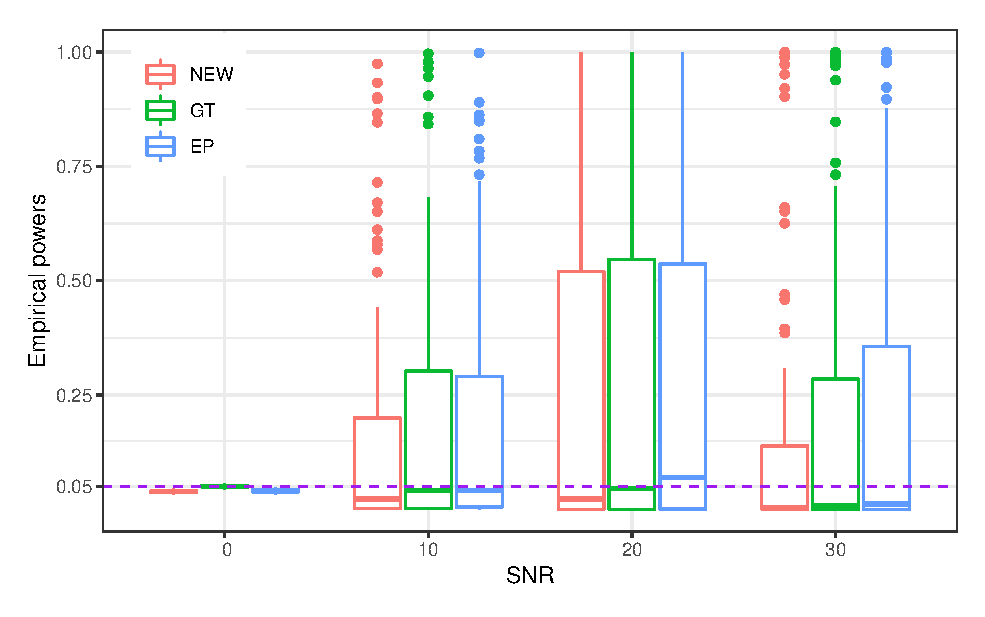
\includegraphics[width=0.45\textwidth]{code/figure/50_iidnormal_t_dense}
    }
    \subfigure[$n=50$, $\epsilon_1\sim t_8$. Sparse $\bbeta_b$.]{
        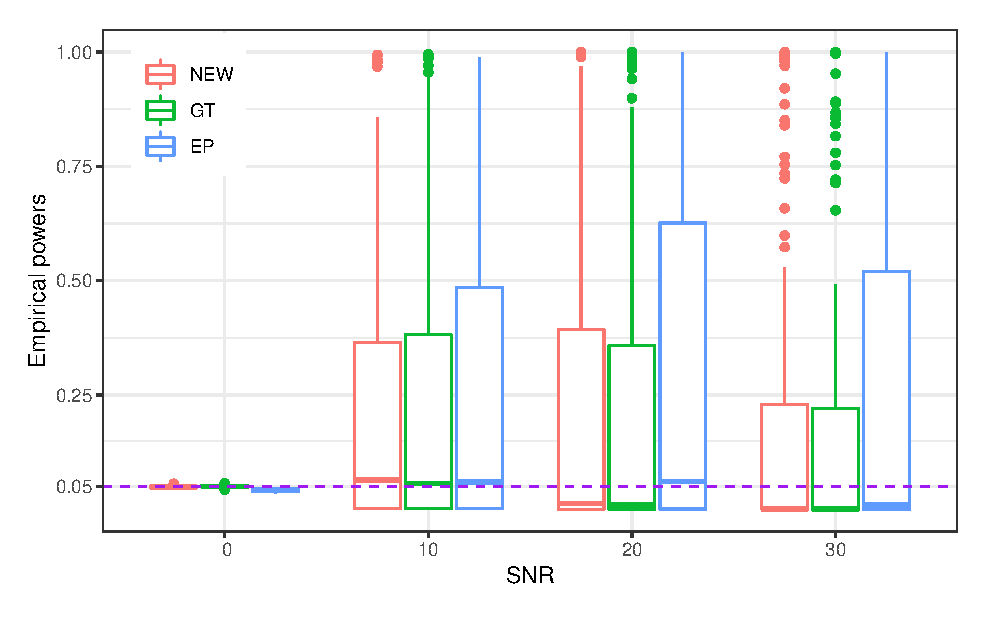
\includegraphics[width=0.45\textwidth]{code/figure/50_iidnormal_t_sparse}
    }
    \\
    \subfigure[$n=50$, $\epsilon_1\sim (\chi^2(4)-4)/\sqrt{8}$. Dense $\bbeta_b$.]{
        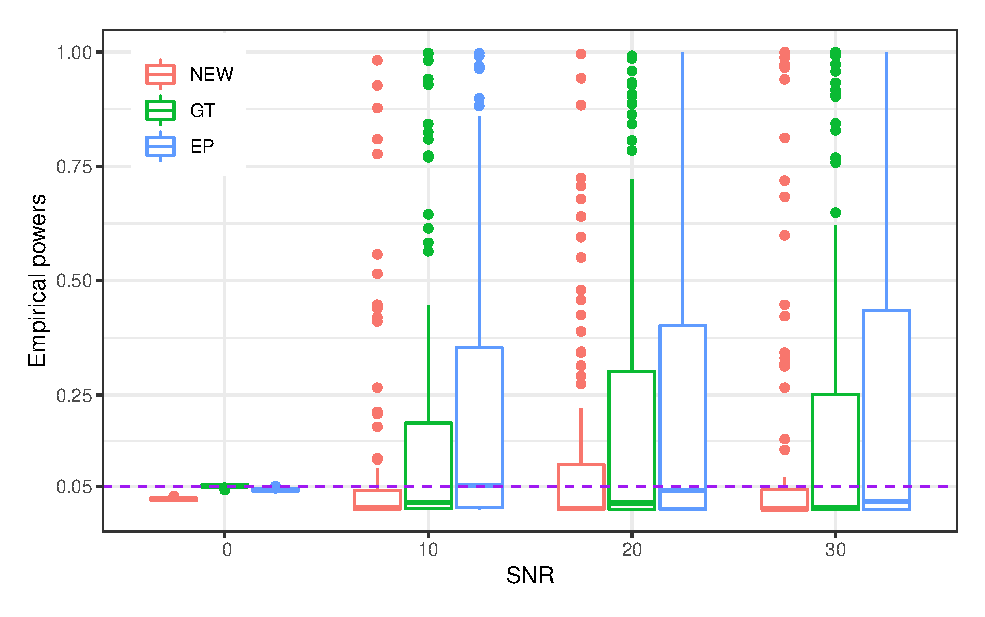
\includegraphics[width=0.45\textwidth]{code/figure/50_iidnormal_chi_dense}
    }
    \subfigure[$n=50$, $\epsilon_1\sim (\chi^2(4)-4)/\sqrt{8}$. Sparse $\bbeta_b$.]{
        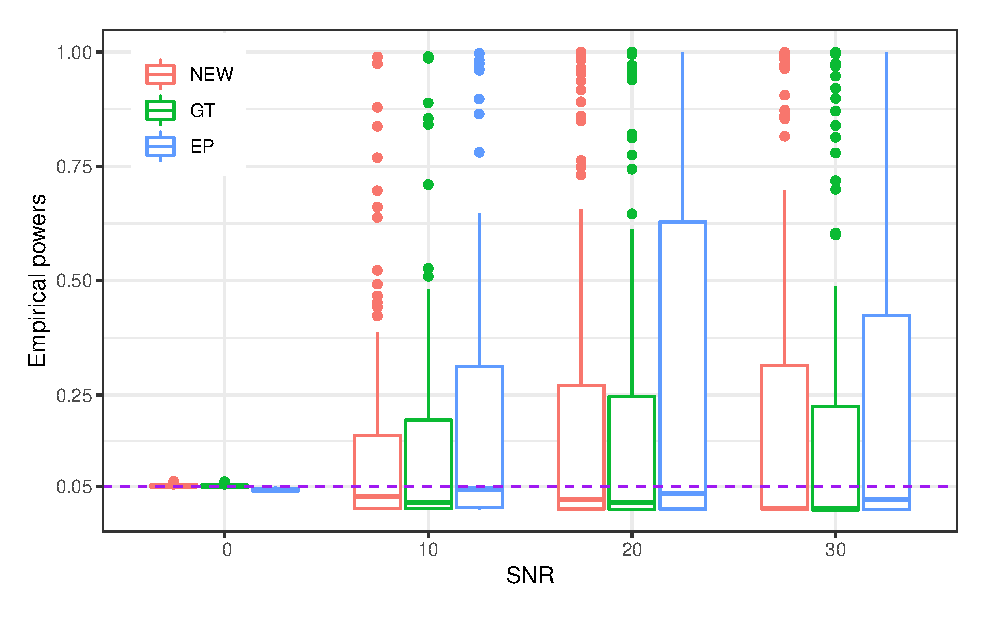
\includegraphics[width=0.45\textwidth]{code/figure/50_iidnormal_chi_sparse}
    }
    \\
    \subfigure[$n=100$, $\epsilon_1\sim t_8$. Dense $\bbeta_b$.]{
        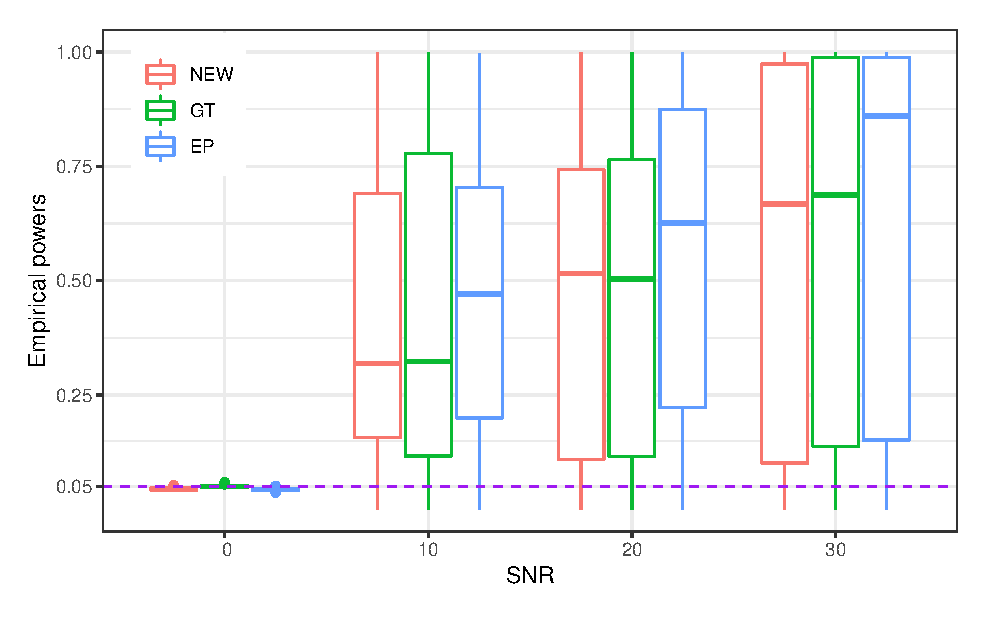
\includegraphics[width=0.45\textwidth]{code/figure/100_iidnormal_t_dense}
    }
    \subfigure[$n=100$, $\epsilon_1\sim t_8$. Sparse $\bbeta_b$.]{
        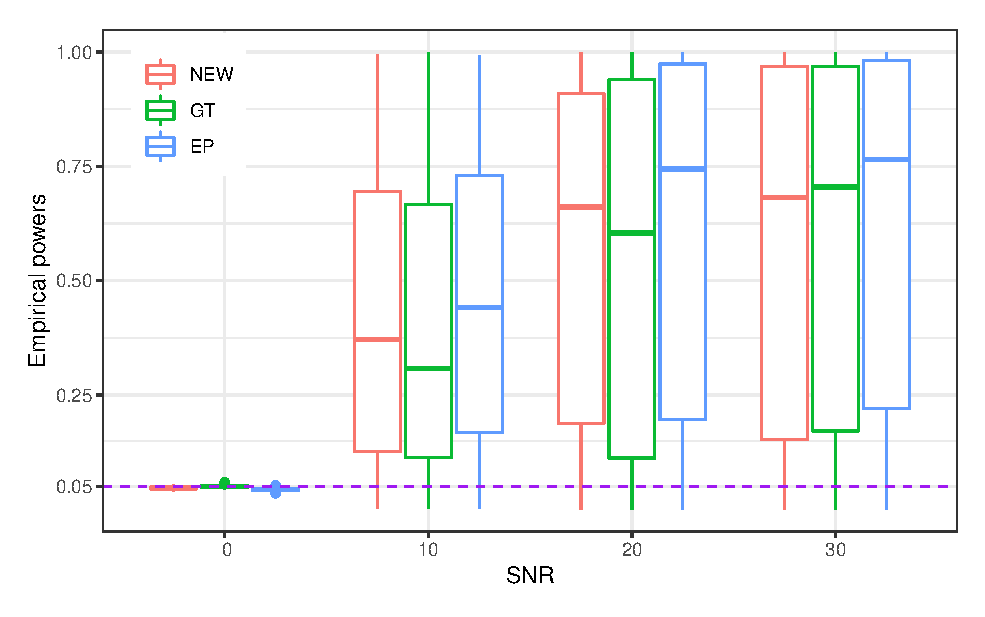
\includegraphics[width=0.45\textwidth]{code/figure/100_iidnormal_t_sparse}
    }
    \\
    \subfigure[$n=100$, $\epsilon_1\sim (\chi^2(4)-4)/\sqrt{8}$. Dense $\bbeta_b$.]{
        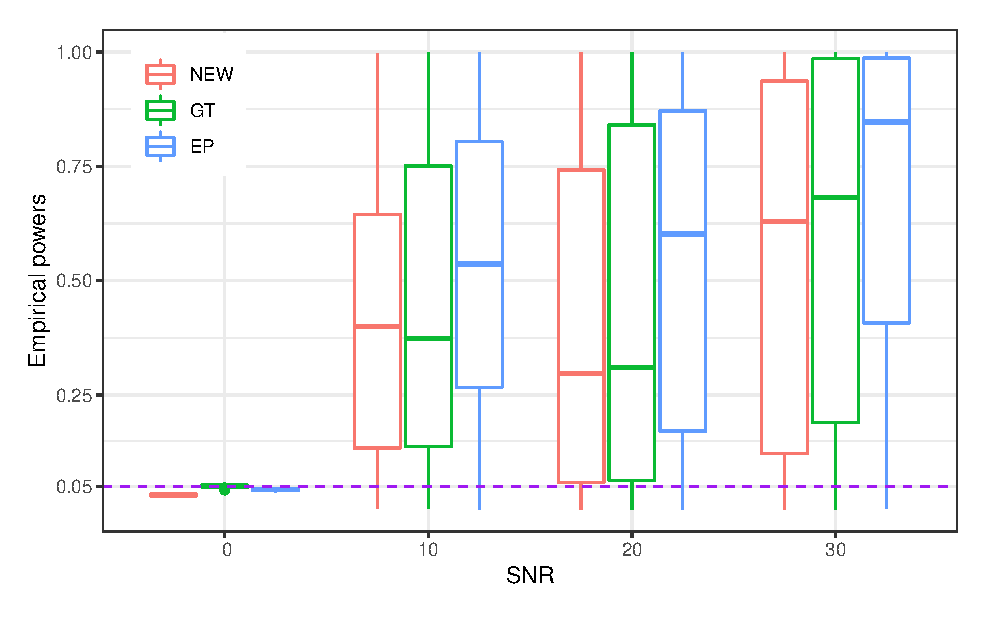
\includegraphics[width=0.45\textwidth]{code/figure/100_iidnormal_chi_dense}
    }
    \subfigure[$n=100$, $\epsilon_1\sim (\chi^2(4)-4)/\sqrt{8}$. Sparse $\bbeta_b$.]{
        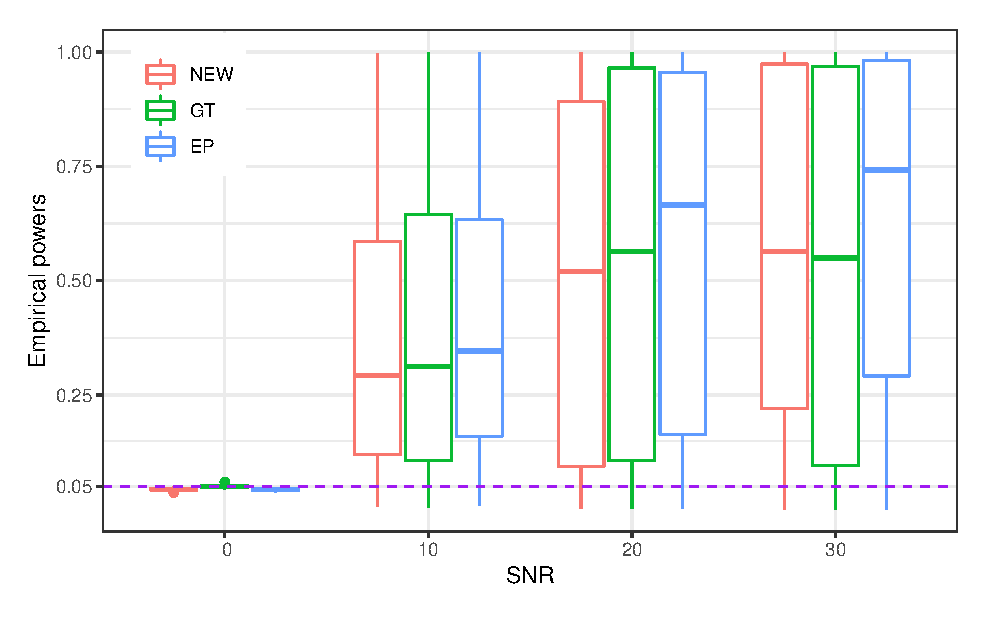
\includegraphics[width=0.45\textwidth]{code/figure/100_iidnormal_chi_sparse}
    }
    \caption{Box plots of the empirical powers based on $25$ independently generated $\bbeta_b$ and $5$,$000$ independent replications.
        Identity covariance matrix.
        $q=10$, $p=1000$, $\alpha=0.05$.
    }\label{fig:1}
\end{figure}

\begin{figure}
    \centering 
    \subfigure[$n=50$, $\epsilon_1\sim t_8$. Dense $\bbeta_b$.]{
        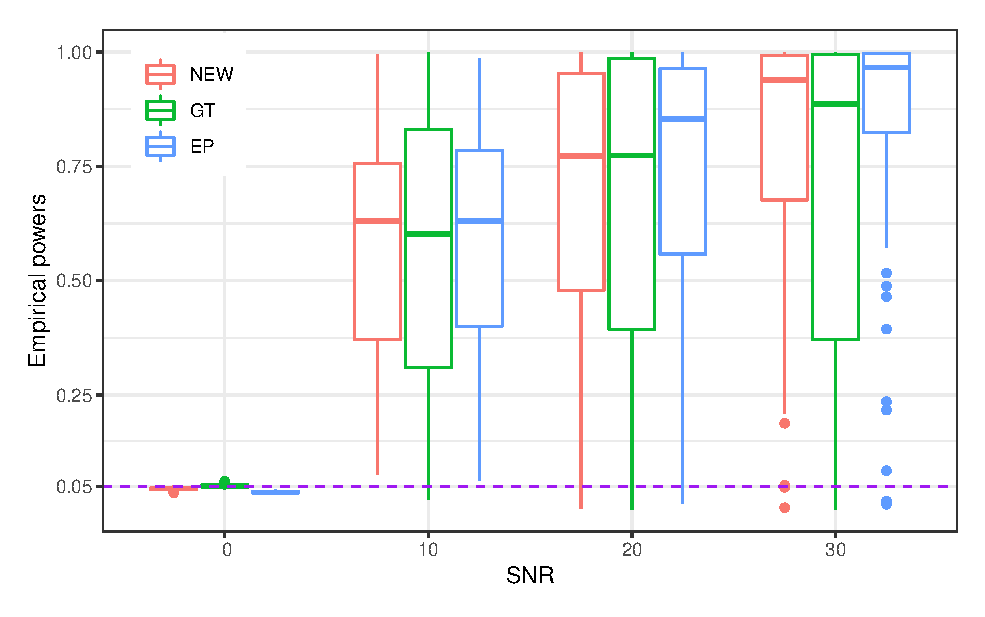
\includegraphics[width=0.45\textwidth]{code/figure/50_Toeplitz_t_dense}
    }
    \subfigure[$n=50$, $\epsilon_1\sim t_8$. Sparse $\bbeta_b$.]{
        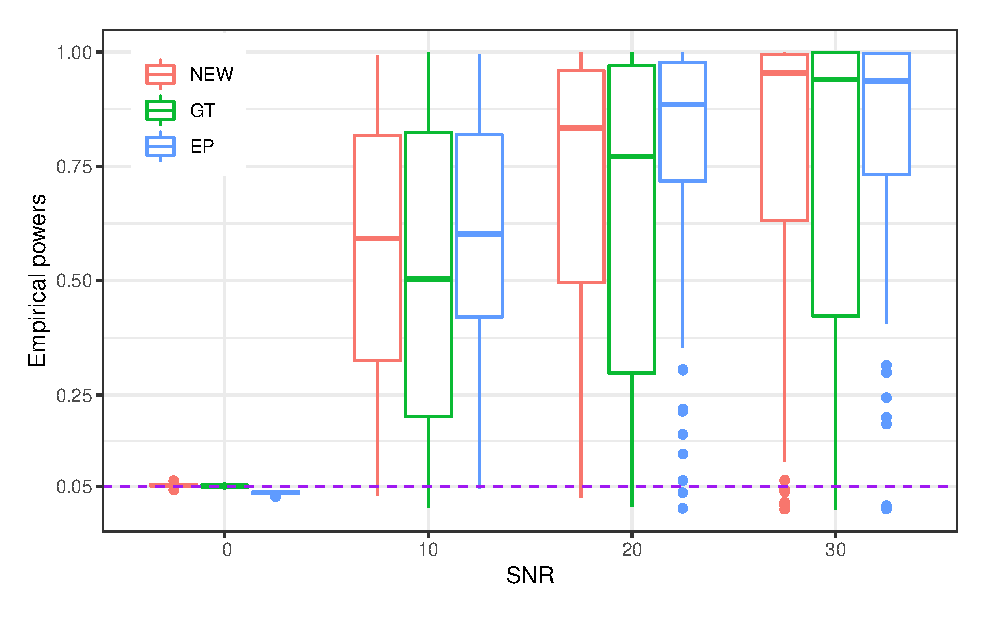
\includegraphics[width=0.45\textwidth]{code/figure/50_Toeplitz_t_sparse}
    }
    \\
    \subfigure[$n=50$, $\epsilon_1\sim (\chi^2(4)-4)/\sqrt{8}$. Dense $\bbeta_b$.]{
        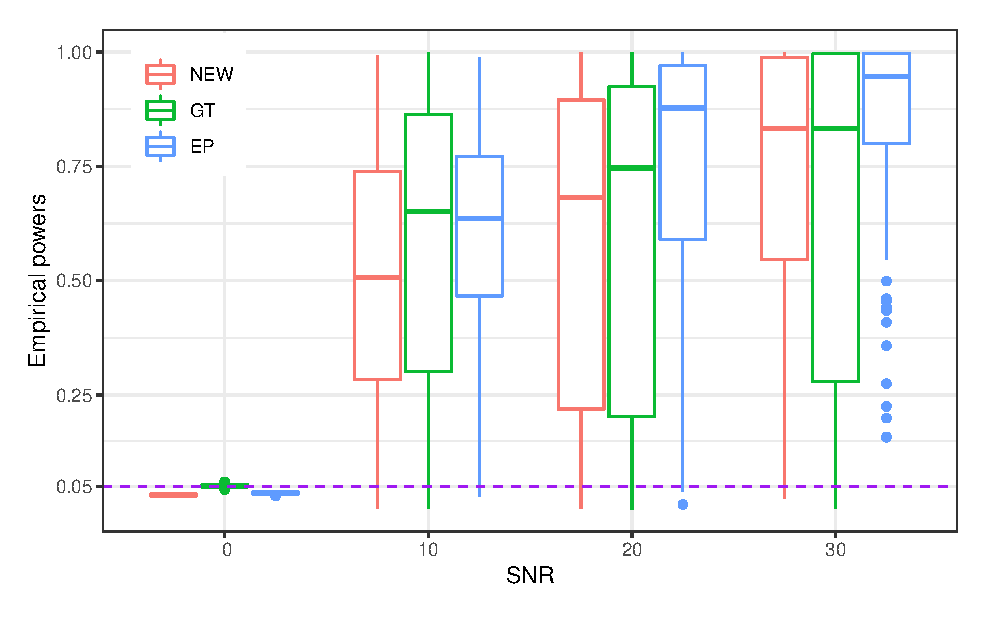
\includegraphics[width=0.45\textwidth]{code/figure/50_Toeplitz_chi_dense}
    }
    \subfigure[$n=50$, $\epsilon_1\sim (\chi^2(4)-4)/\sqrt{8}$. Sparse $\bbeta_b$.]{
        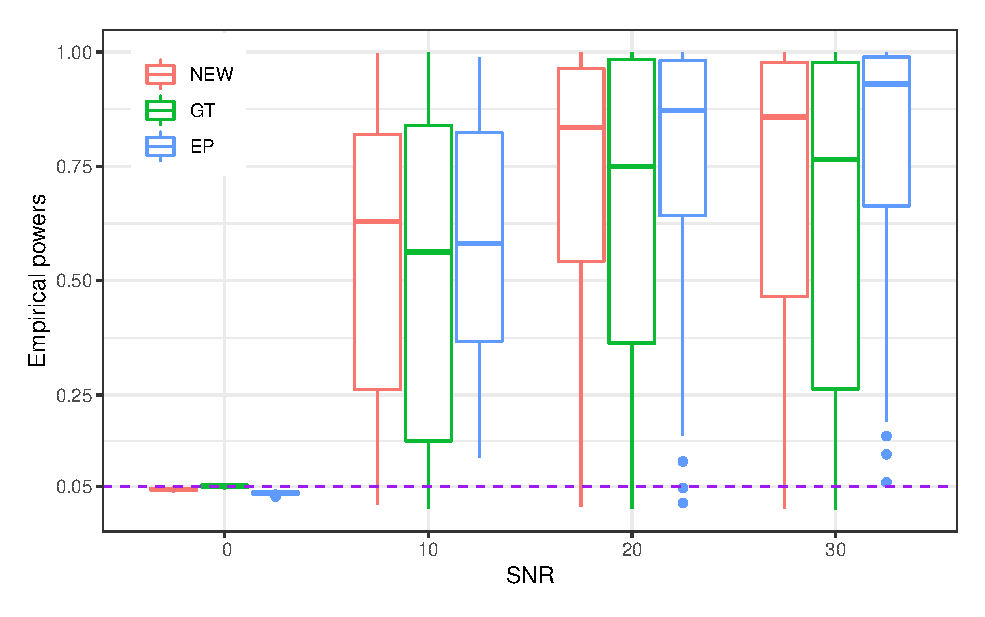
\includegraphics[width=0.45\textwidth]{code/figure/50_Toeplitz_chi_sparse}
    }
    \\
    \subfigure[$n=100$, $\epsilon_1\sim t_8$. Dense $\bbeta_b$.]{
        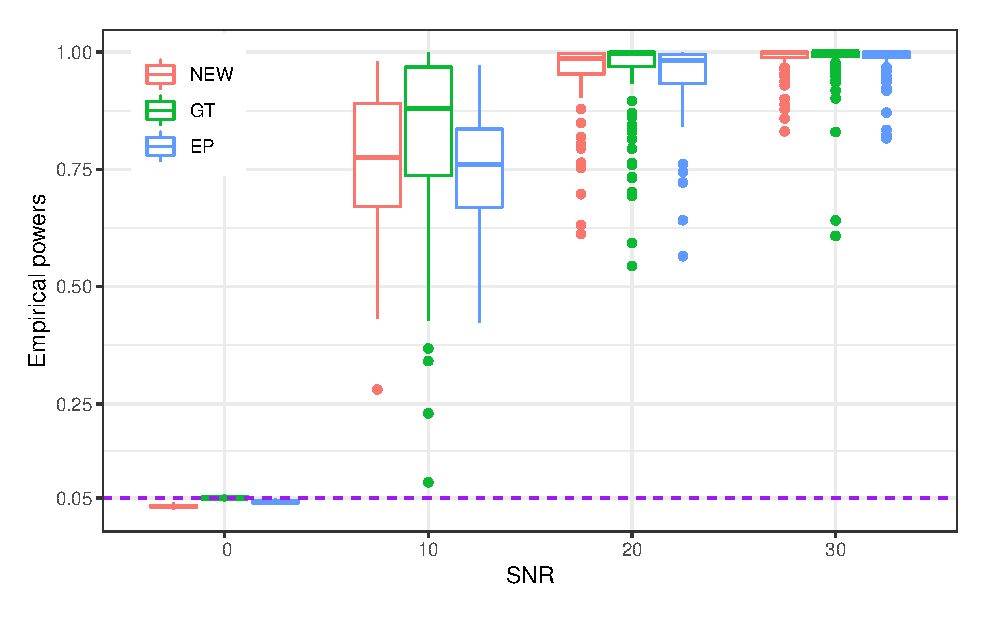
\includegraphics[width=0.45\textwidth]{code/figure/100_Toeplitz_t_dense}
    }
    \subfigure[$n=100$, $\epsilon_1\sim t_8$. Sparse $\bbeta_b$.]{
        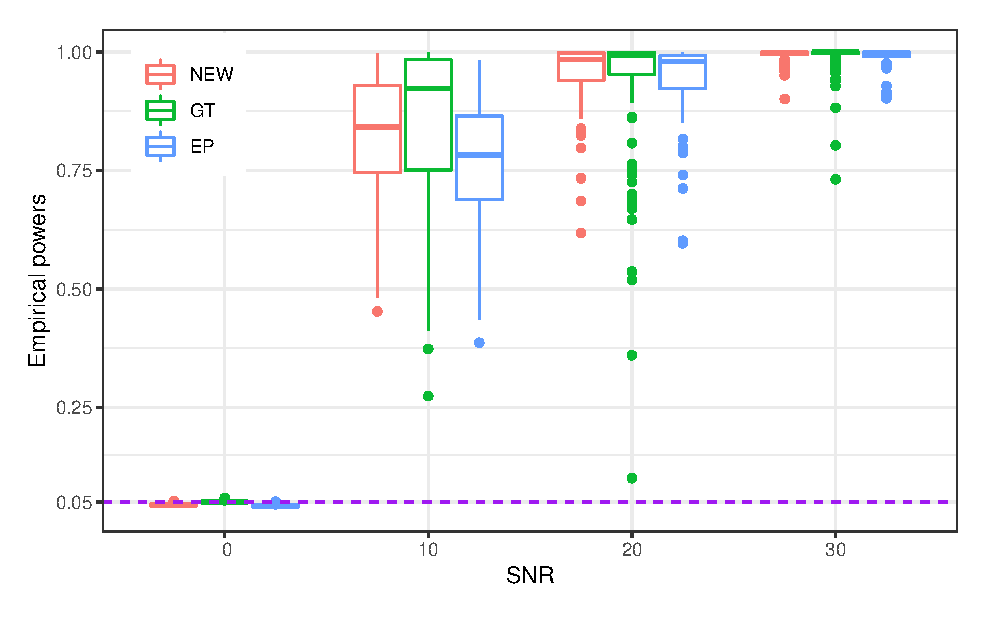
\includegraphics[width=0.45\textwidth]{code/figure/100_Toeplitz_t_sparse}
    }
    \\
    \subfigure[$n=100$, $\epsilon_1\sim (\chi^2(4)-4)/\sqrt{8}$. Dense $\bbeta_b$.]{
        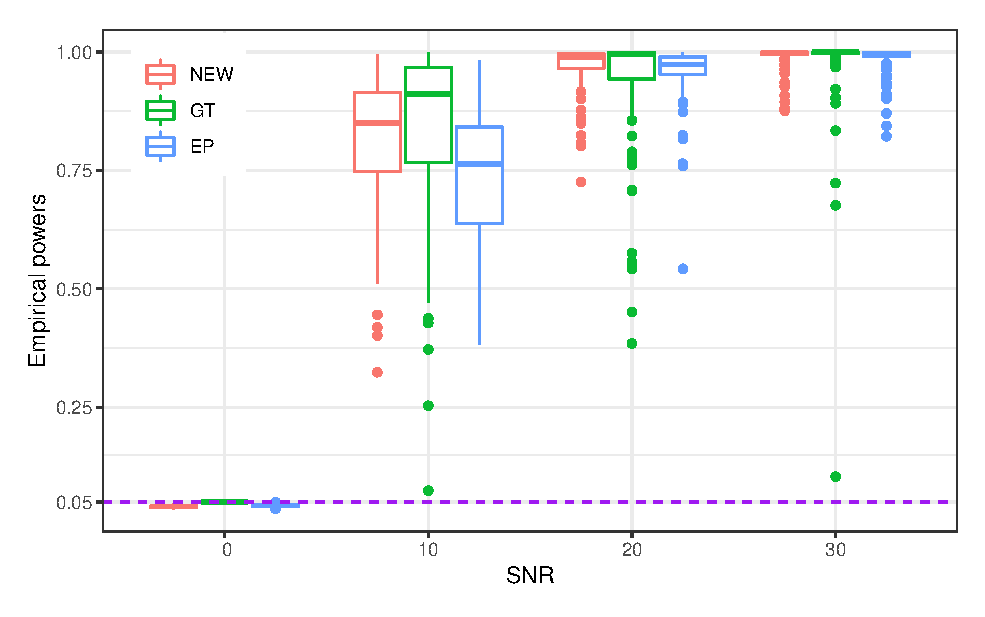
\includegraphics[width=0.45\textwidth]{code/figure/100_Toeplitz_chi_dense}
    }
    \subfigure[$n=100$, $\epsilon_1\sim (\chi^2(4)-4)/\sqrt{8}$. Sparse $\bbeta_b$.]{
        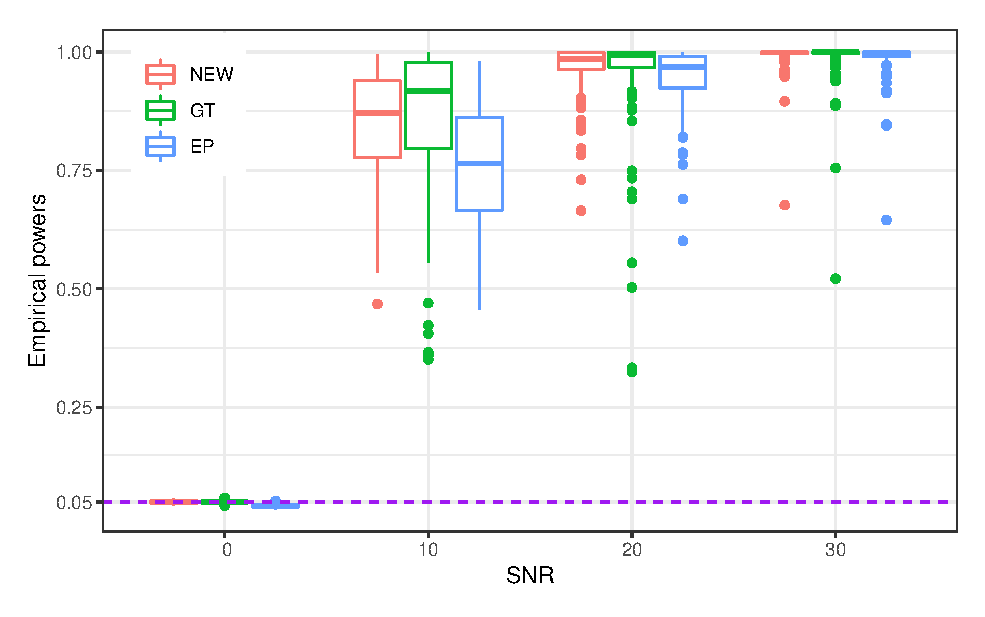
\includegraphics[width=0.45\textwidth]{code/figure/100_Toeplitz_chi_sparse}
    }
    \caption{Box plots of the empirical powers based on $25$ independently generated $\bbeta_b$ and $5$,$000$ independent replications.
Toeplitz covariance matrix.
        $q=10$, $p=1000$, $\alpha=0.05$.
    }\label{fig:2}
\end{figure}

\begin{figure}
    \centering 
    \subfigure[$n=50$, $\epsilon_1\sim t_8$. Dense $\bbeta_b$.]{
        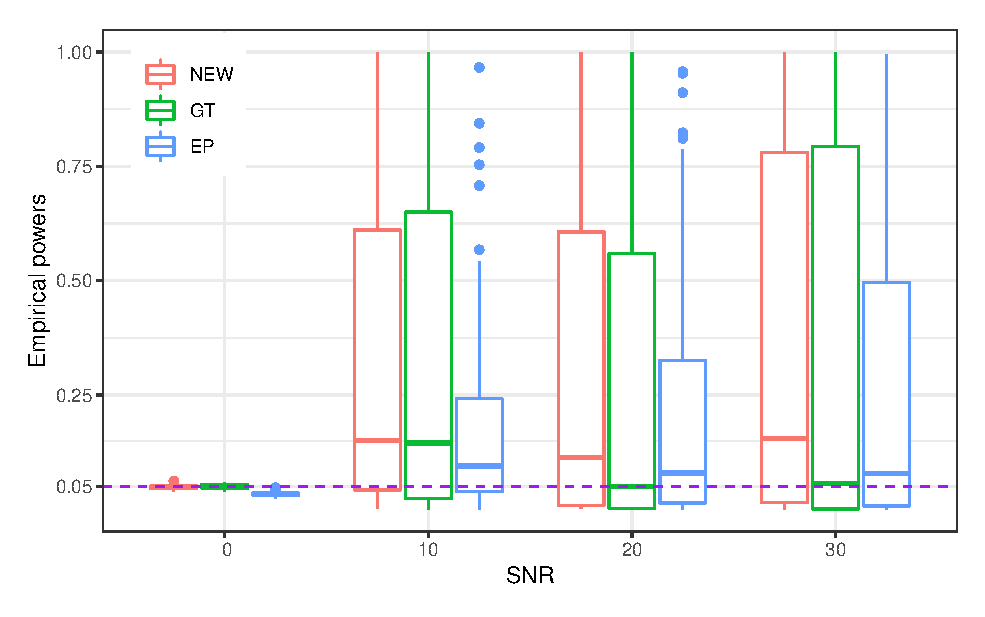
\includegraphics[width=0.45\textwidth]{code/figure/50_equalCor_t_dense}
    }
    \subfigure[$n=50$, $\epsilon_1\sim t_8$. Sparse $\bbeta_b$.]{
        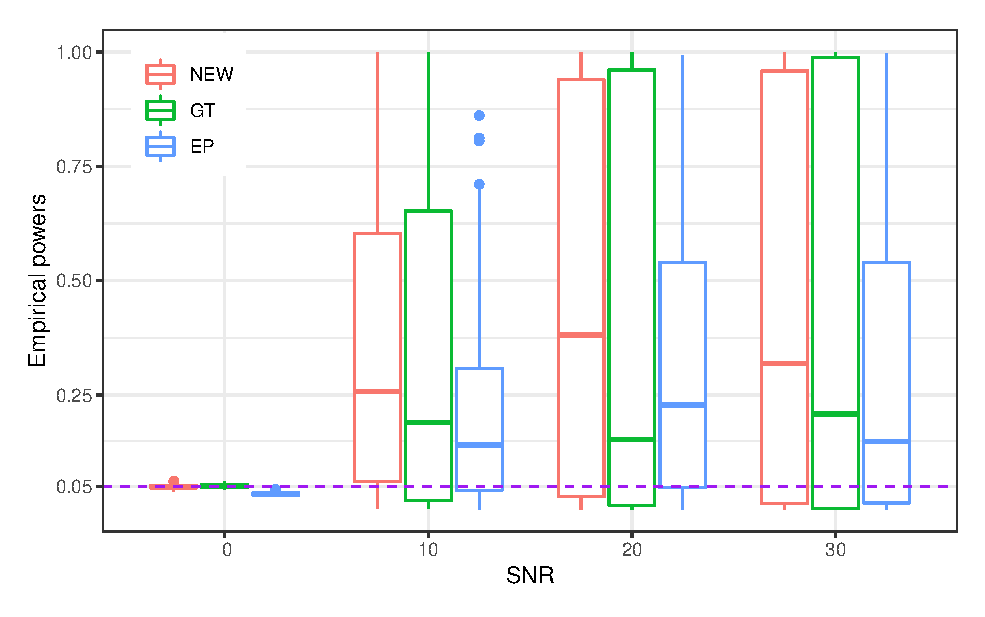
\includegraphics[width=0.45\textwidth]{code/figure/50_equalCor_t_sparse}
    }
    \\
    \subfigure[$n=50$, $\epsilon_1\sim (\chi^2(4)-4)/\sqrt{8}$. Dense $\bbeta_b$.]{
        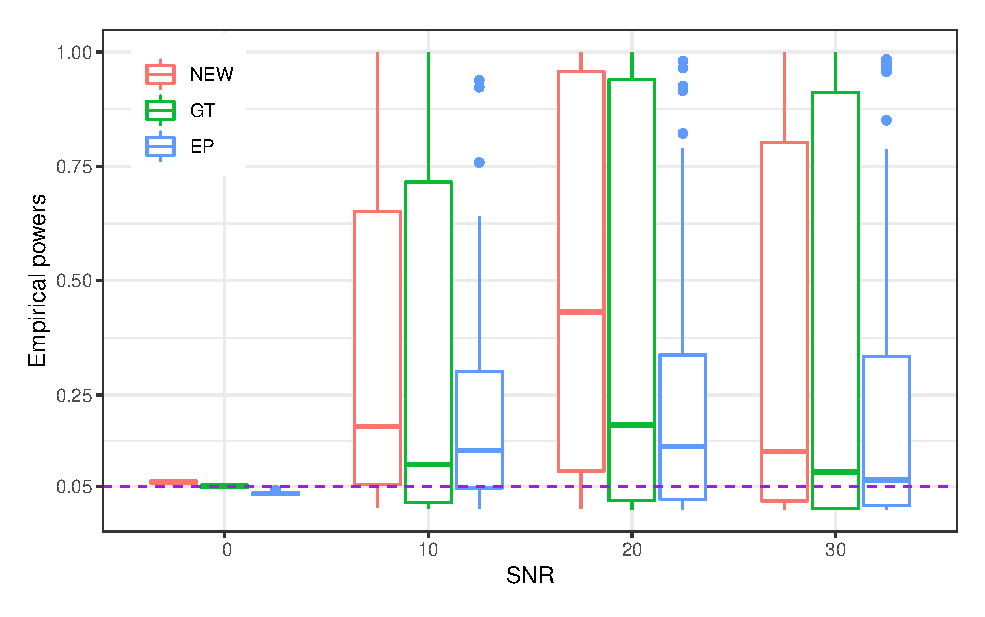
\includegraphics[width=0.45\textwidth]{code/figure/50_equalCor_chi_dense}
    }
    \subfigure[$n=50$, $\epsilon_1\sim (\chi^2(4)-4)/\sqrt{8}$. Sparse $\bbeta_b$.]{
        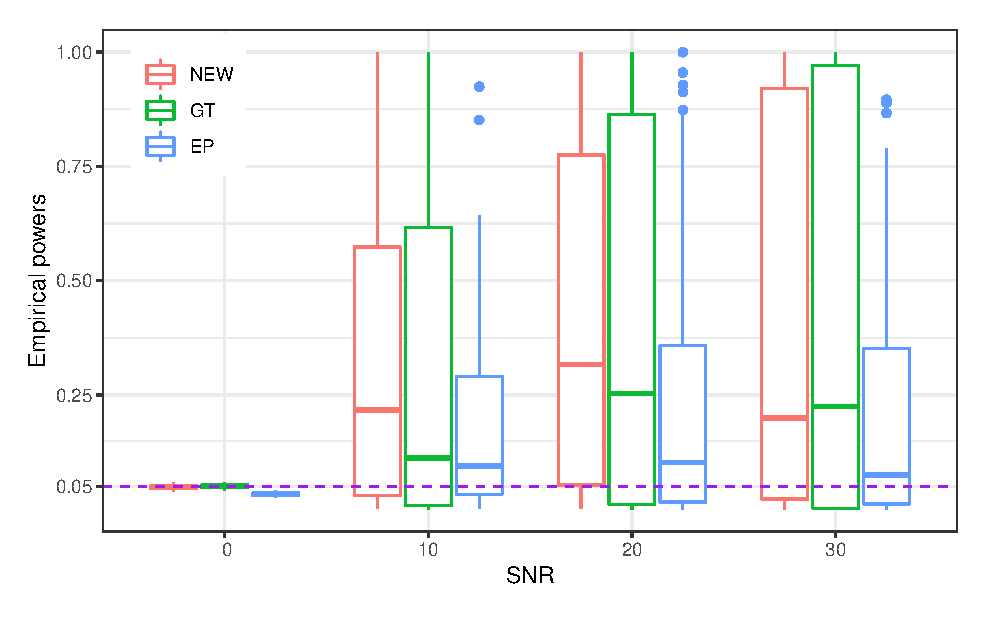
\includegraphics[width=0.45\textwidth]{code/figure/50_equalCor_chi_sparse}
    }
    \\
    \subfigure[$n=100$, $\epsilon_1\sim t_8$. Dense $\bbeta_b$.]{
        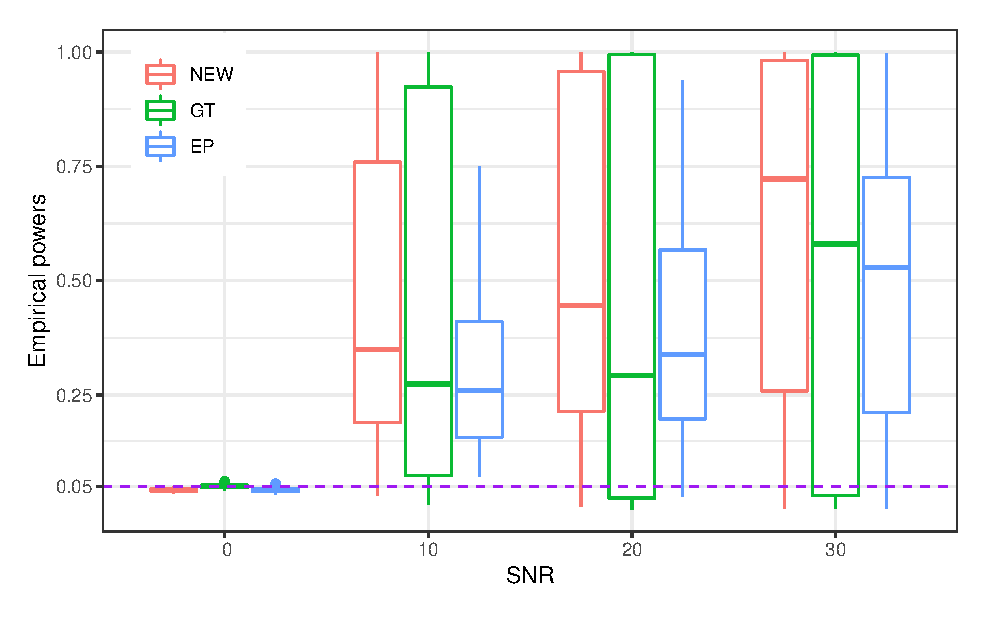
\includegraphics[width=0.45\textwidth]{code/figure/100_equalCor_t_dense}
    }
    \subfigure[$n=100$, $\epsilon_1\sim t_8$. Sparse $\bbeta_b$.]{
        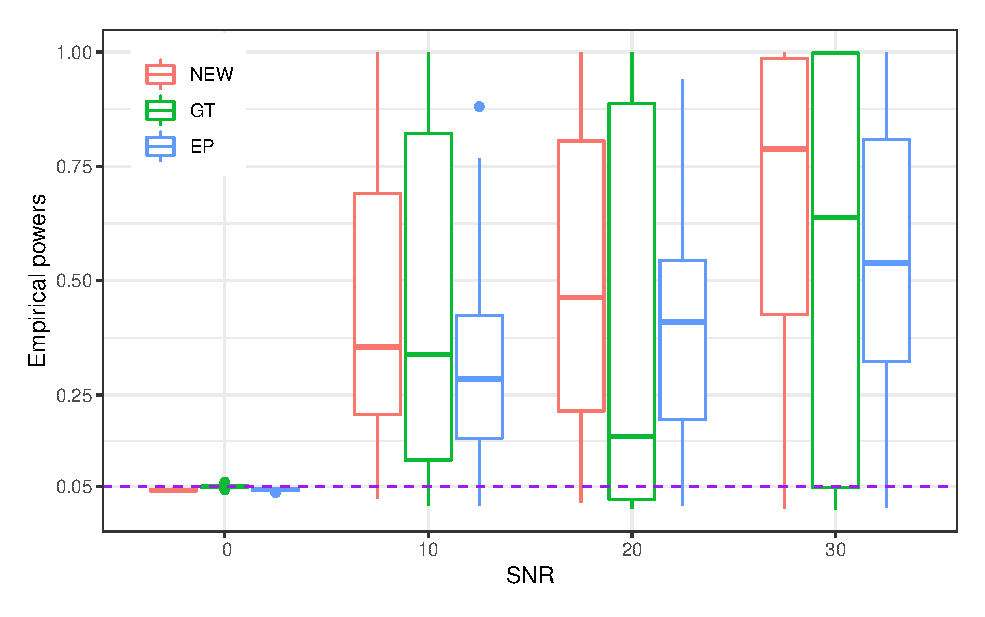
\includegraphics[width=0.45\textwidth]{code/figure/100_equalCor_t_sparse}
    }
    \\
    \subfigure[$n=100$, $\epsilon_1\sim (\chi^2(4)-4)/\sqrt{8}$. Dense $\bbeta_b$.]{
        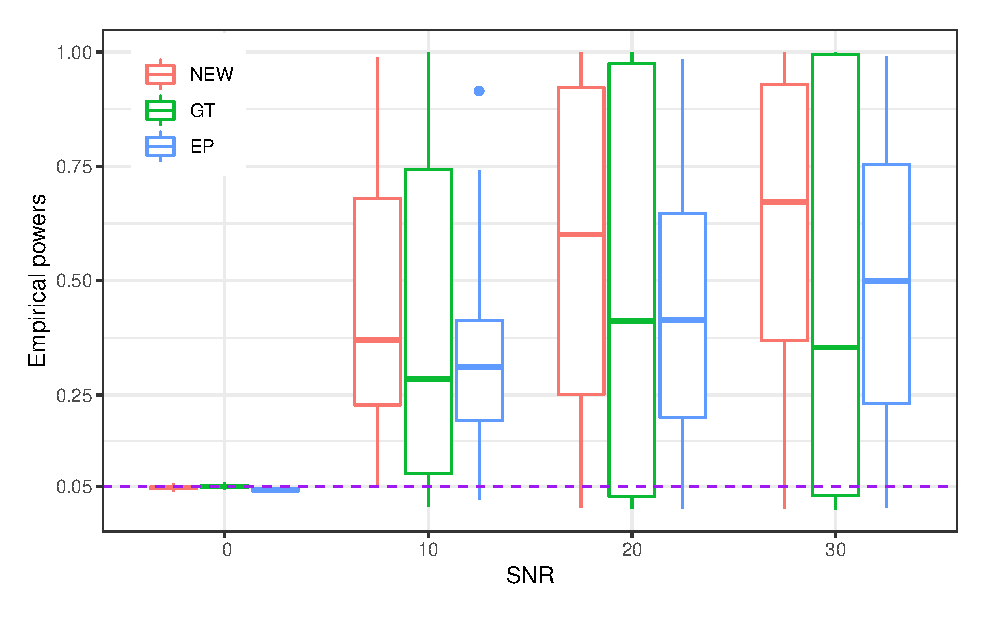
\includegraphics[width=0.45\textwidth]{code/figure/100_equalCor_chi_dense}
    }
    \subfigure[$n=100$, $\epsilon_1\sim (\chi^2(4)-4)/\sqrt{8}$. Sparse $\bbeta_b$.]{
        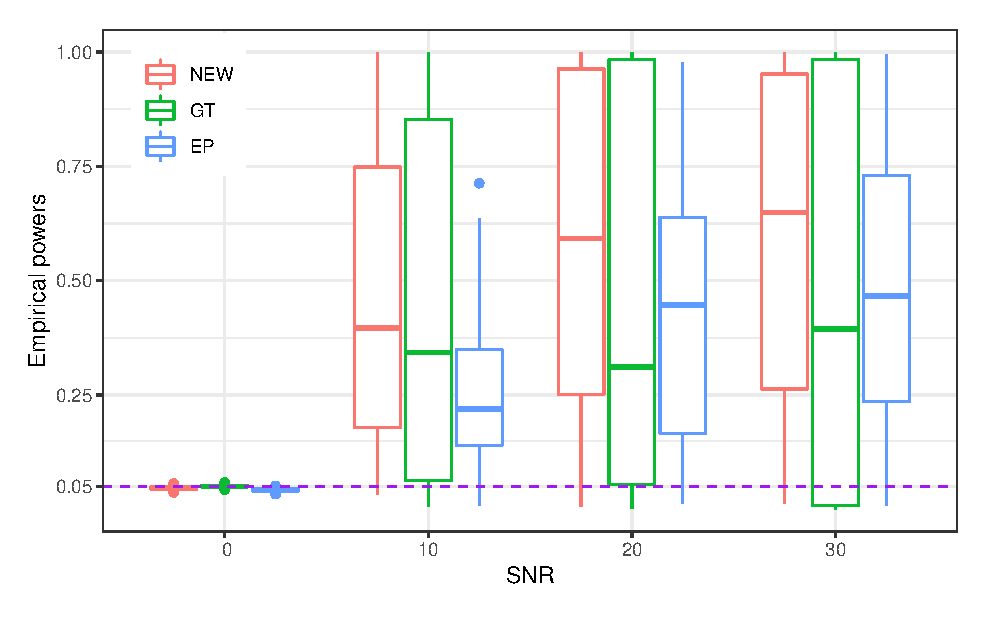
\includegraphics[width=0.45\textwidth]{code/figure/100_equalCor_chi_sparse}
    }
    \caption{Box plots of the empirical powers based on $25$ independently generated $\bbeta_b$ and $5$,$000$ independent replications.
        Equal correlation covariance matrix.
        $q=10$, $p=1000$, $\alpha=0.05$.
    }\label{fig:3}
\end{figure}

%
%\begin{table*}[ht]
%    \caption{
%        Empirical size and power under Toeplitz structure; $q=10$, $p=1000$, $\alpha=0.05$.
%    }
%\label{table1}
%    \centering
%    \begin{tabular}{clcccccccc}
%          \toprule
%          & & \multicolumn{4}{c}{$\epsilon_1\sim t_8$} &\multicolumn{4}{c}{$\epsilon_1\sim (\chi^2(4)-4)/\sqrt{8}$}\\
%          \cmidrule(r){3-6}\cmidrule(r){7-10}
%          & & \multicolumn{2}{c}{Dense $\bbeta_b$} & \multicolumn{2}{c}{Sparse $\bbeta_b$} & \multicolumn{2}{c}{Dense $\bbeta_b$}& \multicolumn{2}{c}{Sparse $\bbeta_b$}\\
%          \cmidrule(r){3-4}  \cmidrule(r){5-6} \cmidrule(r){7-8}  \cmidrule(r){9-10}
%           $n$&SNR & NEW & GT & NEW & GT & NEW & GT & NEW & GT \\ 
%            \midrule
%        $50$ &0 (size)
% & 0.0590 & 0.0546 & 0.0348 & 0.0542 & 0.0346 & 0.0486 & 0.0334 & 0.0498 \\ 
%  &5 & 0.3650 & 0.3438 & 0.2818 & 0.3500 & 0.3474 & 0.3954 & 0.3304 & 0.3786 \\ 
%  &10 & 0.5266 & 0.4850 & 0.4584 & 0.4896 & 0.5036 & 0.5314 & 0.5034 & 0.5396 \\ 
%  &15 & 0.6282 & 0.5654 & 0.5638 & 0.5822 & 0.5812 & 0.5892 & 0.5800 & 0.5884 \\ 
%  &20 & 0.6980 & 0.6114 & 0.6222 & 0.6298 & 0.6390 & 0.6370 & 0.6204 & 0.6192 \\ 
%  &25 & 0.7228 & 0.6412 & 0.6466 & 0.6398 & 0.6610 & 0.6504 & 0.6550 & 0.6374 \\ 
%  &30 & 0.7362 & 0.6418 & 0.6920 & 0.6878 & 0.6932 & 0.6700 & 0.6706 & 0.6518 \\ 
%        \midrule
%$100$&0 (size) 
%& 0.0620 & 0.0510 & 0.0380 & 0.0504 & 0.0530 & 0.0478 & 0.0482 & 0.0514 \\ 
%  &5 & 0.4572 & 0.5056 & 0.3630 & 0.4962 & 0.5534 & 0.6048 & 0.4908 & 0.5988 \\ 
%  &10 & 0.7496 & 0.7664 & 0.6562 & 0.7478 & 0.8404 & 0.8468 & 0.7950 & 0.8198 \\ 
%  &15 & 0.8830 & 0.8658 & 0.8330 & 0.8666 & 0.9296 & 0.9134 & 0.9110 & 0.9066 \\ 
%  &20 & 0.9500 & 0.9176 & 0.9100 & 0.9224 & 0.9660 & 0.9504 & 0.9586 & 0.9506 \\ 
%  &25 & 0.9682 & 0.9460 & 0.9532 & 0.9470 & 0.9832 & 0.9682 & 0.9782 & 0.9656 \\ 
%  &30 & 0.9836 & 0.9604 & 0.9676 & 0.9664 & 0.9924 & 0.9770 & 0.9874 & 0.9730 \\ 
%        \bottomrule
%    \end{tabular}
%\end{table*}
%
%\begin{table*}[ht]
%    \caption{
%        Empirical size and power under equal correlation structure; $q=10$, $p=1000$, $\alpha=0.05$.
%    }
%\label{table2}
%    \centering
%    \begin{tabular}{clcccccccc}
%          \toprule
%          & & \multicolumn{4}{c}{$\epsilon_1\sim t_8$} &\multicolumn{4}{c}{$\epsilon_1\sim (\chi^2(4)-4)/\sqrt{8}$}\\
%          \cmidrule(r){3-6}\cmidrule(r){7-10}
%          & & \multicolumn{2}{c}{Dense $\bbeta_b$} & \multicolumn{2}{c}{Sparse $\bbeta_b$} & \multicolumn{2}{c}{Dense $\bbeta_b$}& \multicolumn{2}{c}{Sparse $\bbeta_b$}\\
%          \cmidrule(r){3-4}  \cmidrule(r){5-6} \cmidrule(r){7-8}  \cmidrule(r){9-10}
%           $n$&SNR & NEW & GT & NEW & GT & NEW & GT & NEW & GT \\ 
%            \midrule
%        $50$ &0 (size)
%& 0.0458 & 0.0492 & 0.0464 & 0.0502 & 0.0524 & 0.0530 & 0.0520 & 0.0516 \\ 
%  &5 & 0.2524 & 0.2594 & 0.2640 & 0.2674 & 0.2634 & 0.2630 & 0.2914 & 0.2836 \\ 
%  &10 & 0.3228 & 0.3102 & 0.3396 & 0.3278 & 0.3316 & 0.3070 & 0.3758 & 0.3432 \\ 
%  &15 & 0.3530 & 0.3382 & 0.3732 & 0.3520 & 0.3598 & 0.3332 & 0.3960 & 0.3654 \\ 
%  &20 & 0.3754 & 0.3498 & 0.3862 & 0.3644 & 0.3628 & 0.3320 & 0.4146 & 0.3728 \\ 
%  &25 & 0.3872 & 0.3566 & 0.4022 & 0.3694 & 0.3810 & 0.3394 & 0.4228 & 0.3822 \\ 
%  &30 & 0.4130 & 0.3736 & 0.4006 & 0.3684 & 0.3830 & 0.3478 & 0.4352 & 0.3930 \\ 
%        \midrule
%$100$&0 (size) 
% & 0.0458 & 0.0540 & 0.0482 & 0.0462 & 0.0406 & 0.0526 & 0.0464 & 0.0480 \\ 
%  &5 & 0.2472 & 0.3176 & 0.2570 & 0.3158 & 0.2914 & 0.3584 & 0.3142 & 0.3496 \\ 
%  &10 & 0.3818 & 0.4078 & 0.3950 & 0.4108 & 0.4298 & 0.4482 & 0.4582 & 0.4402 \\ 
%  &15 & 0.4820 & 0.4720 & 0.4788 & 0.4594 & 0.5172 & 0.5008 & 0.5542 & 0.4820 \\ 
%  &20 & 0.5292 & 0.4900 & 0.5414 & 0.4928 & 0.5742 & 0.5212 & 0.5988 & 0.5090 \\ 
%  &25 & 0.5700 & 0.5040 & 0.5984 & 0.5200 & 0.6018 & 0.5338 & 0.6262 & 0.5164 \\ 
%  &30 & 0.5972 & 0.5202 & 0.6172 & 0.5296 & 0.6392 & 0.5508 & 0.6582 & 0.5336 \\ 
%        \bottomrule
%    \end{tabular}
%\end{table*}
%
%\begin{table*}[ht]
%    \caption{
%        Empirical size and power under the design matrix of Bacillus subtilis gene expression data; $n=71$, $q=10$, $p=4078$, $\alpha=0.05$.
%    }
%\label{table3}
%    \centering
%    \begin{tabular}{lcccccccc}
%          \toprule
%           & \multicolumn{4}{c}{$\epsilon_1\sim t_8$} &\multicolumn{4}{c}{$\epsilon_1\sim (\chi^2(4)-4)/\sqrt{8}$}\\
%          \cmidrule(r){2-5}\cmidrule(r){6-9}
%           & \multicolumn{2}{c}{Dense $\bbeta_b$} & \multicolumn{2}{c}{Sparse $\bbeta_b$} & \multicolumn{2}{c}{Dense $\bbeta_b$}& \multicolumn{2}{c}{Sparse $\bbeta_b$}\\
%          \cmidrule(r){2-3}  \cmidrule(r){4-5} \cmidrule(r){6-7}  \cmidrule(r){8-9}
%           SNR & NEW & GT & NEW & GT & NEW & GT & NEW & GT \\ 
%            \midrule
%         0 (size) &0.0368 & 0.0524 & 0.0362 & 0.0450 & 0.0378 & 0.0538 & 0.0412 & 0.0534 \\ 
%  5 & 0.1720 & 0.3516 & 0.1804 & 0.3710 & 0.2322 & 0.4134 & 0.2380 & 0.4108 \\ 
%  10 & 0.3268 & 0.4884 & 0.3542 & 0.5128 & 0.4108 & 0.5428 & 0.4206 & 0.5496 \\ 
%  15 & 0.4588 & 0.5624 & 0.4746 & 0.5742 & 0.5512 & 0.6224 & 0.5618 & 0.6168 \\ 
%  20 & 0.5716 & 0.6366 & 0.5636 & 0.6154 & 0.6586 & 0.6690 & 0.6516 & 0.6606 \\ 
%  25 & 0.6398 & 0.6546 & 0.6370 & 0.6578 & 0.7258 & 0.6984 & 0.7318 & 0.6968 \\ 
%  30 & 0.7052 & 0.6802 & 0.7132 & 0.6864 & 0.7872 & 0.7242 & 0.7932 & 0.7248 \\ 
%        \bottomrule
%    \end{tabular}
%\end{table*}
%









\section{Conclusions}\label{sec:conclusions}
We have proposed a Bayesian-motivated test statistic for high-dimensional linear model with fixed design.
We proposed an approximation of the null distribution of the proposed test statistic which is then used to determine the critical value of the test statistic.
Under weak conditions, we proved the proposed test procedure is asymptotically level $\alpha$.
Under certain conditions, we also derived the asymptotic power function of the proposed test.
The proposed test is powerful especially when the signal is strong.

In Theorem \ref{TheoremLindeberg}, we assumed that the distribution of $\epsilon_1$ is symmetric about $0$. 
This condition is also assumed by \cite{Bai2017} in the study of central limit theorem of quadratic form.
Without this condition, our proof of Theorem \ref{TheoremLindeberg} is not valid.
We think it will be an interesting and useful work to relax the symmetric condition in Theorem \ref{TheoremLindeberg}.



\section*{Acknowledgments}
This work was supported by the National Natural Science Foundation of China under Grant No.\ 11471035.





\appendix
\section*{Appendix}

\begin{lemma}\label{Lemma:FF}
    Under the assumptions of Proposition \ref{prop:unbiased}, if there exists a Borel set $G\subset \mathbb R^n$ and a number $M\geq 0$ such that 
    \begin{equation*}
        \int_{\mathbb R^n} \varphi(\By) d\mathcal N_n(\mu,\phi^{-1} \BI_n)(\By)\, \mathrm{d} \By \geq \alpha\quad \text{for all $\mu \in G$ and $\phi >M$},
    \end{equation*}
    then $\lambda(\{\By : \phi(\By)< \alpha, \By \in G\})=0$.
\end{lemma}
\begin{proof}
    %Next we prove $\varphi(\By) \geq \alpha$, a.s.\ $\lambda$ by contradiction.
    We prove the claim by contradiction.
    Suppose $\lambda(\{\By:\varphi (\By) <\alpha,\, \By \in G\})>0$.
    Then there exists a sufficiently small $0< \eta <\alpha$, such that $\lambda(\{\By:\varphi (\By) <\alpha-\eta,\, \By \in G\})>0$.
    We denote $ E:=\{\By\in \mathbb R^n:\varphi (\By) <\alpha-\eta,\,  \By \in G\}$.
    From Lebesgue density theorem \citep[Corollary 6.2.6]{book:992991}, there exists a point $z\in  E$, such that, for any $\varepsilon >0$ there is a $\delta_{\varepsilon}>0$ such that for any $0 < \delta' <\delta_\varepsilon$,
    \begin{equation*}
        \left|\frac{\lambda(E^\complement\cap C_{\delta'})}{\lambda(C_{\delta'})}\right|<\varepsilon,
    \end{equation*}
    where $C_{\delta'}=\prod_{i=1}^n [z_i-{\delta'}, z_i + {\delta'}]$.
    We put
    \begin{equation*}
        \varepsilon=\left(\frac{\sqrt \pi}{\sqrt 2 \Phi^{-1}\left(1-\frac{\eta}{6n}\right)}\right)^n \frac{\eta}{3},
    \end{equation*}
    where $\Phi(\cdot)$ is the cumulative distribution function of a standard normal random variable.
    Then for any $\phi>M$ and $0<\delta' <\delta_\varepsilon$,
    \begin{equation*}
        \begin{split}
            \alpha \leq& 
            \int_{\mathbb R^n}\varphi(\By) d\mathcal N_n (z, \phi^{-1} \BI_n) (\By)\,\mathrm{d} \By
            \\
            =&
            \int_{E\cap C_{\delta'}}\varphi(\By) d\mathcal N_n (z, \phi^{-1} \BI_n) (\By)\,\mathrm{d} \By
            +
            \int_{E^\complement\cap C_{\delta'}}\varphi(\By) d\mathcal N_n (z, \phi^{-1} \BI_n) (\By)\,\mathrm{d} \By
            \\
            &+
            \int_{C_{\delta'}^\complement}\varphi(\By) d\mathcal N_n (z, \phi^{-1} \BI_n) (\By)\,\mathrm{d} \By
            \\
            \leq&
            \alpha-\eta
            +
            \int_{E^\complement\cap C_{\delta'}} d\mathcal N_n (z, \phi^{-1} \BI_n) (\By)\,\mathrm{d} \By
            +
            \int_{C_{\delta'}^\complement} d\mathcal N_n (z, \phi^{-1} \BI_n) (\By)\,\mathrm{d} \By
            \\
            \leq&
            \alpha-\eta
            +
            \left(\frac{\phi}{2\pi}\right)^{n/2}\lambda(E^\complement\cap C_{\delta'})
            +
            2n\left(1-\Phi(\sqrt \phi \delta')\right)
            \\
            \leq&
            \alpha-\eta
            +
            \left(\frac{\phi}{2\pi}\right)^{n/2}
            \varepsilon
            (2\delta')^n
            +
            2n\left(1-\Phi(\sqrt \phi \delta')\right)
            \\
            =&
            \alpha-\eta
            +
            \left(\frac{\sqrt{\phi} \delta'}{\Phi^{-1}\left(1-\frac{\eta}{6n}\right)}\right)^{n}
            \frac{\eta}{3}
            +
            2n\left(1-\Phi(\sqrt \phi \delta')\right).
        \end{split}
    \end{equation*}
    In the last inequality, we put $\delta'$ small enough such that
\begin{equation*}
    \left(\frac{\Phi^{-1}\left(1-\frac{\eta}{6n}\right)}{\delta'}\right)^2>M,
\end{equation*}
and put
    \begin{equation*}
        \phi = \left(\frac{\Phi^{-1}\left(1-\frac{\eta}{6n}\right)}{\delta'}\right)^2.
    \end{equation*}
    Then we obtain the contradiction $\alpha\leq \alpha-(2/3)\eta$.
    This completes the proof.

    
\end{proof}

\begin{proof}[\textbf{Proof of Proposition \ref{prop:unbiased}}]
    
    To prove the claim (a), 
    %Since $\myRank([\BX_a,\BX_b])=n$,
    note that $\varphi(\By)$ is unbiased if and only if
    \begin{equation*}
        \int_{\mathbb R^n} \varphi(\By) d\mathcal N_n (\mu,\phi^{-1} \BI_n) (\By) \,\mathrm{d} \By\geq \alpha
        \quad \text{for all $\mu\in \mathbb R^n$ and $\phi>0$}.
    \end{equation*}
    %where $\mathcal N_n(\mu,\sigma^2 \BI_n)(d\By)$ is the density function of a $\mathcal N_n (\mu, \sigma^2 \BI_n)$ random vector with respect to Lebesgue measure $\lambda(\cdot)$.
    Then Lemma \ref{Lemma:FF} implies that $\varphi(\By) \geq \alpha$, a.s.\ $\lambda$.
    %From \cite{Lehmann}, Theorem 2.7.1, $\myE [\varphi(\By)]=\alpha$ under the null hypothesis.
    %In particular,
    %we have
    On the other hand, since $\varphi(\By)$ is a level $\alpha$ test, for every $\phi>0$,
    \begin{equation}\label{eq:unbiasedproof1}
        \int_{\mathbb R^n} [\varphi(\By)-\alpha] d\mathcal N_n (0,\phi^{-1} \BI_n)(\By) \,\mathrm{d} \By\leq 0.
    \end{equation}
    Note that the integrand of \eqref{eq:unbiasedproof1} is nonnegative. Hence $\varphi(\By)-\alpha=0$ a.s.\ $\lambda$.
    This proves the claim (a). 

    Now we prove the claim (b) by contradiction.
    Suppose
    \begin{equation*}
        \int_{\mathbb R^n} \varphi(\By) d\mathcal N_n \left(\BX_a \bbeta_a + \BX_b \bbeta_b,\phi^{-1} \BI_n\right) (\By)\, \mathrm{d}\By 
        \geq \alpha 
    \end{equation*}
    for every $\bbeta_a\in \mathbb R^q$, $\bbeta_b \in \mathbb R^p$, $\phi>0$ satisfying $h(\phi) \bbeta_b^\top \BX_b^\top (\BI_n - \BP_a) \BX_b \bbeta_b >M$.
    Since $h(\phi)$ is nondecreasing, there exists a number $M^* >0$ such that
    \begin{equation*}
        \left\{(\bbeta_b^\top, \phi)^\top :  \bbeta_b^\top \BX_b^\top (\BI_n - \BP_a) \BX_b \bbeta_b >M^*,\phi>M^* \right\} 
        \subset
        \left\{(\bbeta_b^\top, \phi)^\top :  h(\phi)\bbeta_b^\top \BX_b^\top (\BI_n - \BP_a) \BX_b \bbeta_b > M^*\right\} .
    \end{equation*}
    Then Lemma \ref{Lemma:FF} implies that $\varphi(\By) \mathbf 1_{G}(\By)\geq \alpha \mathbf 1_{G}(\By)$ a.e.\ $\lambda$, where 
    \begin{equation*}
        G=\left\{ \BX_a \bbeta_a + \BX_b \bbeta_b:  \bbeta_a \in \mathbb R^{q},
        \bbeta_b^\top \BX_b^\top (\BI_n - \BP_a) \BX_b \bbeta_b >M^*
    \right\}.
    \end{equation*}
    It can be easily seen that
    \begin{equation*}
        G=\left\{
            w+z: w\in \textrm{span}(\BX_a), z \in \textrm{span}(\BX_a)^{\bot},
            \|z\| > M^*
        \right\},
    \end{equation*}
    where $\textrm{span}(\BX_a)$ is the linear span of the columns of $\BX_a$ and $\textrm{span}(\BX_a)^\bot$ is the orthogonal complement of $\textrm{span}(\BX_a)$.
    Since $\varphi(\By)$ is nonrandom and $\alpha>0$, we have $\varphi(\By) \mathbf 1_{G}(\By)\geq \mathbf 1_{G}(\By)$ a.e.\ $\lambda$.
    Also note that $\varphi(\By)$ is a level $\alpha$ test, then for every $\phi>0$, we have
    \begin{equation*}
        \begin{split}
            \alpha \geq&
        \int_{\mathbb R^n} \varphi(\By) d\mathcal N_n (0,\phi^{-1} \BI_n)(\By) \,\mathrm{d} \By
        \\
        \geq& 
        \int_{G} d\mathcal N_n (0,\phi^{-1} \BI_n)(\By) 
        \\
        =&\Pr\left( 
            R > \phi M^{*2}
        \right),
        \end{split}
    \end{equation*}
    where $R$ is a random variable with distribution $\chi^2(n-q)$.
    Thus, we obtain a contradiction by letting $\phi\to 0$ in the above inequality.
    This completes the proof.

\end{proof}





\begin{proof}[\textbf{Proof of Theorem \ref{TheoremLindeberg}}]
    Let
    \begin{equation*}
        \tilde a_{i,j}:=
        \frac{a_{i,j}}{
            \sqrt{
    2\mytr(\BA^2)
    +
    (\myE(\xi_1^4)-3)\mytr(\BA^{\circ 2} )
            }             
        }
        .
    \end{equation*}
Then
    \begin{equation*}
        S=\sum_{i=1}^n \tilde a_{i,i}(\xi_i^2-1)
        +2\sum_{1\leq i < j \leq n}  \tilde a_{i,j} \xi_i \xi_j,
\quad
        S_\tau^* =\tau \sum_{i=1}^n \tilde a_{i,i}\check z_i
        +2\sum_{1\leq i <j \leq n} \tilde a_{i,j} z_i z_j.
    \end{equation*}
    For $l=1,\ldots, n$, define
    \begin{align*}
        S_l = & 
        \sum_{i=1}^{l-1} \tilde a_{i,i}(\xi_i^2-1)
        +
        \tau\sum_{i=l+1}^{n} \tilde a_{i,i}  \check  z_i
        +2\sum_{1\leq i <j \leq l-1}  \tilde a_{i,j} \xi_i \xi_j
        +2\sum_{i=1}^{l-1} \sum_{j=l+1}^n \tilde a_{i,j} \xi_i z_j
        +2\sum_{l+1 \leq i < j \leq n}  \tilde a_{i,j} z_i z_j
        ,
        \\
        h_l = & \tilde a_{l,l} (\xi_l^2 -1)
        +2\sum_{i=1}^{l-1} \tilde a_{i,l} \xi_i \xi_l
        +2\sum_{i =l +1}^n \tilde a_{i,l} z_i \xi_l
        ,
        \\
        g_l = &
        \tau \tilde a_{l,l} \check z_l
        +2\sum_{i =1}^{l-1} \tilde a_{i,l} \xi_i z_l
        +2\sum_{i = l+1}^n \tilde a_{i,l} z_i z_l
        .
    \end{align*}
    It can be seen that for $l=2,\ldots, n$, 
    $S_{l-1}+ h_{l-1} =S_{l} + g_{l} $, and
    $S=S_n + h_n$, $S_1 + g_1=S_\tau^*$.
    %\begin{equation*}
        %S_n + h_n =  \sum_{i=1}^n \tilde a_{i,i}(\xi_i^2 - 1)
        %+2 \sum_{1\leq i < j \leq n} \tilde a_{i,j} \xi_i \xi_j,
    %\end{equation*}
    %\begin{equation*}
        %S_1 + g_1 = \sum_{i=1}^n \tilde a_{i,i}\check z_i
        %+2\sum_{1\leq i <j \leq n} \tilde a_{i,j} z_i z_j.
    %\end{equation*}

    Thus, for any $f \in \mathscr C^4 (\mathbb R)$,
    \begin{equation*}
        \begin{split}
        \left|\myE f\left(S\right)
        -
        \myE f\left(S_\tau^*\right)\right| 
        =&
        \left| \myE f(S_n+h_n)-\myE f(S_1+g_1)\right|
        \\
        =&
        \left|\sum_{l=2}^{n} \left(\myE f(S_{l}+h_{l})-\myE f(S_{l-1}+h_{l-1})\right)+\myE f(S_{1}+h_{1})-\myE f(S_{1}+g_{1})\right|
        \\
        = &
       \left| \sum_{l=1}^{n} \myE f(S_{l}+h_{l})-\myE f(S_{l}+g_{l})\right|
       .
        \end{split}
    \end{equation*}
    Apply Taylor's theorem, for $l=1,\ldots,n$,
    \begin{equation*}
        \begin{split}
            f(S_{l}+h_{l})=&
            f(S_{l})
            +
            \sum_{k=1}^3
            \frac{1}{k!} h_l^k f^{(k)} (S_{l})
            +
            \frac{1}{24}h_{l}^4 f^{(4)} (S_{l}+\theta_1 h_{l}),
            \\
            f(S_{l}+g_{l})=&
            f(S_{l})
            +
            \sum_{k=1}^3
            \frac{1}{k!} g_l^k f^{(k)} (S_{l})
            +
            \frac{1}{24}g_{l}^4 f^{(4)} (S_{l}+\theta_{2} g_{l}),
        \end{split}
    \end{equation*}
    where $\theta_1,\theta_2\in[0,1]$.
    Thus,
    \begin{equation*}
        \begin{split}
             &\left| \myE f(S_{l}+h_{l})-\myE f(S_{l}+g_{l})\right|
\leq
\left|
            \sum_{k=1}^3
            \frac{1}{k!} \myE f^{(k)} (S_{l})
            \myE_l (h_l^k - g_l^k)
            \right|
            +
            \frac{1}{24} \|f'''' \|_{\infty} \left(\myE (h_{l}^4)+\myE (g_{l}^4)\right),
        \end{split}
    \end{equation*}
where $\myE_l$ denotes taking expectation with respect to $\xi_l, z_l ,\check z_l$.
It is straightforward to show that
\begin{equation*}
    \begin{split}
        \myE_l (h_l-g_l)&=0, 
        \\
        \myE_l (h_l^2-g_l^2)&= 
        \left(
            \myE (\xi_1^4) - 1
            -
            \tau^2
        \right)
        \tilde a_{l,l}^2
        ,
        \\
        \myE_l (h_l^3-g_l^3)&= 
        \myE (\xi_1^2-1)^3
        \tilde a_{l,l}^3 
        +
        12 (\myE (\xi_1^4) - 1) \tilde a_{l,l} \left( \sum_{i=1}^{l-1} \tilde a_{i,l} \xi_i + \sum_{i=l+1}^n \tilde a_{i,l} z_i    \right)^2 
        .
    \end{split}
\end{equation*}
Thus,
\begin{equation}\label{eq:Lin1}
        \begin{split}
             &\left| \myE f(S_{l}+h_{l})-\myE f(S_{l}+g_{l})\right|
             \\
\leq&
\frac{1}{2}
\|f^{(2)}\|_\infty
\left|
\myE(\xi_1^4)-1
            -\tau^2
\right|
        \tilde a_{l,l}^2
        \\
            &+
            \frac{1}{6} \|f^{(3)}\|_{\infty}
\left(
    \left|\myE (\xi_1^2-1)^3\right|
        |\tilde a_{l,l}^3 |
        +
        12 (\myE (\xi_1^4)-1) |\tilde a_{l,l}|
            \myE 
            \left( \sum_{i=1}^{l-1} \tilde a_{i,l} \xi_i + \sum_{i=l+1}^n \tilde a_{i,l} z_i    \right)^2 
    \right)
    \\
            &+
            \frac{1}{24} \|f^{(4)} \|_{\infty} \left(\myE (h_{l}^4)+\myE (g_{l}^4)\right)
            \\
\leq &
\frac{
\left|
\myE (\xi_1^4)-1
            -
            \tau^2
\right|
}{2}
\|f^{(2)}\|_\infty
        \tilde a_{l,l}^2
            +
            \frac{
            \max\left(
    \left|\myE (\xi_1^2-1)^3\right|
            ,
12 (\myE (\xi_1^4)-1)
        \right)
            }{6} \|f^{(3)}\|_\infty
|\tilde a_{l,l}|
         \sum_{i=1}^{n} \tilde a_{i,l}^2 
         \\
            &+
            \frac{1}{24} \|f^{(4)} \|_{\infty} \left(\myE (h_{l}^4)+\myE (g_{l}^4)\right)
            .
        \end{split}
    \end{equation}
    Now we bound $\myE (h_l^4)$ and $\myE (g_l^4)$.
    By direct calculation,
\begin{equation*}
    \begin{split}
        \myE (h_l^4)
        =&
        \myE (\xi_1^2 - 1)^4 \tilde a_{l,l}^4
        + 24 \myE [ \xi_1^2(\xi_1^2 -1)^2]
        \tilde a_{l,l}^2
        \myE \left( 
        \sum_{i=1}^{l-1} \tilde a_{i,l} \xi_i 
        +\sum_{i =l +1}^n \tilde a_{i,l} z_i 
        \right)^2
        \\
        &+
        16 \myE (\xi_1^4 )
        \myE \left( 
        \sum_{i=1}^{l-1} \tilde a_{i,l} \xi_i 
        +\sum_{i =l +1}^n \tilde a_{i,l} z_i 
    \right)^4
    \\
    =&
        \myE (\xi_1^2 - 1)^4 \tilde a_{l,l}^4
        + 24 \myE [ \xi_1^2(\xi_1^2 -1)^2]
        \tilde a_{l,l}^2
    \left((\sum_{i=1}^n \tilde a_{i,l}^2) - \tilde a_{l,l}^2\right)
        \\
        &+
        16 \myE (\xi_1^4 )
    \left(
        \left(\myE (\xi_1^4) - 3\right)\sum_{i=1}^{l-1} \tilde a_{i,l}^4 
        + 3 \left( (\sum_{i=1}^n \tilde a_{i,l}^2) - \tilde a_{l,l}^2 \right)^2
    \right)
    .
    \end{split}
\end{equation*}
To upper bound the above quantity, we use the facts
$
24 \myE [ \xi_1^2(\xi_1^2 -1)^2]
\leq 
2(16\myE (\xi_1^2 -1)^4 + (9/4) \myE  (\xi_1^4) )
$,
$\myE (\xi_1^2 - 1)^4\leq \myE (\xi_1^8)$ and
\begin{equation*}
        \left(\myE (\xi_1^4) - 3\right)\sum_{i=1}^{l-1} \tilde a_{i,l}^4 
        \leq
        \left(\myE (\xi_1^4) - 1\right)\sum_{i=1}^{l-1} \tilde a_{i,l}^4 
        \leq
        \left(\myE (\xi_1^4) - 1\right)
        \left( (\sum_{i=1}^n \tilde a_{i,l}^2) - \tilde a_{l,l}^2 \right)^2
        .
\end{equation*}
Then we obtain the bound 
\begin{equation}\label{eq:Lin2}
\myE (h_l^4) \leq \left(16 \myE (\xi_1^8) + 32 \myE (\xi_1^4)\right) \left(\sum_{i=1}^n \tilde a_{i,l}^2\right)^2.
\end{equation}
Similarly, we have
\begin{equation}\label{eq:Lin3}
\myE (g_l^4) \leq \left(  48 \myE (\xi_1^4) + 3\tau^4 + 96 \right) \left(\sum_{i=1}^n \tilde a_{i,l}^2\right)^2.
\end{equation}
Combining \eqref{eq:Lin1}, \eqref{eq:Lin2} and \eqref{eq:Lin3} yields

%It can be seen that
%\begin{align*}
        %\myE \left( 
        %\sum_{i=1}^{l-1} \tilde a_{i,l} \xi_i 
        %+\sum_{i =l +1}^n \tilde a_{i,l} z_i 
        %\right)^2
        %=&\left(\sum_{i=1}^n \tilde a_{i,l}^2\right) - \tilde a_{l,l}^2
        %,
    %\end{align*}
    %and
    %\begin{align*}
        %\myE \left( 
        %\sum_{i=1}^{l-1} \tilde a_{i,l} \xi_i 
        %+\sum_{i =l +1}^n \tilde a_{i,l} z_i 
        %\right)^4
        %=&
        %\left(\myE (\xi_i^4) - 3\right)\sum_{i=1}^{l-1} \tilde a_{i,l}^4 
        %+ 3 \left( \left(\sum_{i=1}^n \tilde a_{i,l}^2\right) - \tilde a_{l,l}^2 \right)^2
        %\\
        %\leq &
        %\left(
         %\myE (\xi_i^4)
     %+ 2\right) \left( \left(\sum_{i=1}^n \tilde a_{i,l}^2\right) - \tilde a_{l,l}^2 \right)^2.
%\end{align*}
    \begin{equation*}
        \begin{split}
             &
             \sum_{l=1}^n \left| \myE f(S_{l}+h_{l})-\myE f(S_{l}+g_{l})\right|
             \\
\leq&
\frac{
\left|
\myE (\xi_1^4)-1
            -
            \tau^2
\right|
}{2}
\|f^{(2)}\|_\infty
\sum_{l=1}^n \tilde a_{l,l}^2
            +
            \frac{
            \max\left(
    \left|\myE (\xi_1^2-1)^3\right|
            ,
12 (\myE (\xi_1^4)-1)
        \right)
            }{6} \|f^{(3)}\|_\infty
            \sum_{l=1}^n 
            \left(|\tilde a_{l,l}|
         \sum_{i=1}^{n} \tilde a_{i,l}^2 
     \right)
         \\
            &+
            \frac{
             16 \myE (\xi_1^8) + 80 \myE (\xi_1^4) + 3\tau^4 + 96 
            }{24} \|f^{(4)} \|_{\infty} 
            \sum_{l=1}^n \left( \sum_{i=1}^n \tilde a_{i,l}^2 \right)^2
            .
        \end{split}
    \end{equation*}
    This completes the proof.
 
\end{proof}


\begin{proof}[\textbf{Proof of Theorem \ref{thm:criticalValue}}]
    Throughout the proof, we use the similar notations as in Theorem \ref{approximation} and define
    \begin{equation*}
        S=\frac{
            (\sqrt \phi \bepsilon)^\top \BA \sqrt \phi \bepsilon - \mytr (\BA)
        }{
            \sqrt{
    2 \mytr(\BA^2)
    +
    (\phi^2\myE (\epsilon_1^4)-3) \mytr(\BA^{\circ 2})
            }             
        }
    \end{equation*}
    and
    \begin{equation*}
        S_{ \hat \tau}^* =
        \frac{
            \hat \tau \sum_{i=1}^n  a_{i,i}\check z_i
        +2\sum_{1\leq i <j \leq n} a_{i,j} z_i z_j
    }
    {
            \sqrt{
    2 \mytr(\BA^2)
    +
    (\phi^2\myE (\epsilon_1^4)-3) \mytr(\BA^{\circ 2})
            }             
        },
    \end{equation*}
    where $z_1,\ldots, z_n, \check z_1,\ldots, \check z_n$ are iid $\mathcal N(0,1)$ random variables and are independent of $\hat \tau^2$.


    By a standard subsequence argument, we only need to prove the theorem along a subsequence of $\{n\}$.
    Hence, without loss of generality, we assume $\hat \tau^2 \xrightarrow{a.s.} \phi^2 \myE (\epsilon_1^4)-1$.
    Write
    \begin{equation*}
        \begin{split}
        S_{\hat \tau}^* =&
        \frac{
            \sqrt{\phi^2\myE (\epsilon_1^4)-1} \sum_{i=1}^n  a_{i,i}\check z_i
        +2\sum_{1\leq i <j \leq n} a_{i,j} z_i z_j
    }
    {
            \sqrt{
    2 \mytr(\BA^2)
    +
    (\phi^2\myE (\epsilon_1^4)-3) \mytr(\BA^{\circ 2})
            }             
        }
        +
        \frac{
                (\hat \tau -
            \sqrt{
                \phi^2\myE (\epsilon_1^4)-1
            }
        )
             \sum_{i=1}^n  a_{i,i}\check z_i
    }
    {
            \sqrt{
    2 \mytr(\BA^2)
    +
    (\phi^2\myE (\epsilon_1^4)-3) \mytr(\BA^{\circ 2})
            }             
        }
        \\
        =:& S_{\hat \tau,1}^{*} + S_{\hat \tau,2}^{*}
    .
        \end{split}
    \end{equation*}
    Note that $S_{\hat{\tau},1}^*$ is independent of $\hat \tau$.
    Since $\myE ( S_{\hat \tau,1}^{*2} )=1$,  the distributions $\mathcal L(S_{\hat \tau,1}^{*}) $ are tight as $n\to \infty$.
    Hence, without loss of generality, we assume $\mathcal L (S_{\hat \tau,1}^*)$ weakly converges to a limit distribution with distribution function $F^\dagger(x)$.
    Let $S^\dagger$ be a random variable with distribution function $F^\dagger(x)$.
    By some algebra (See, e.g., \cite{chen2010tests}, Proposition A.1.(iii)),
    it can be shown that $\myE (S^{*4}_{\hat \tau,1})$ is uniformly bounded.
    Then $\mathcal L ( S_{\hat \tau,1}^{*2} )$ is  uniformly integrable.
    Hence $\myE(S^{\dagger 2})=1$ and $F^\dagger(x)$ can not concentrate on a single point.
    Consequently, $F^\dagger(x)$ is continuous and is strict increasing for $x\in\{x:0<F(x)<1\}$; see \cite{Sevast1961A} as well as the remark made by A. N. Kolmogorov.

    The condition \eqref{eq:jianchiCondition} implies that $\myE[S_{\hat \tau,2}^{*2}|\hat \tau]\to 0$ almost surely.
    Then almost surely, $\mathcal L (S^*_{\hat \tau}|\hat \tau) \rightsquigarrow \mathcal L(S^\dagger)$.
    Consequently, for every $f\in \mathscr C^4 (\mathbb R)$,
    we have $| \myE [f(S^*_{\hat \tau}) |\hat\tau] - \myE f(S^\dagger) |\to 0$ almost surely.
    On the other hand, Theorem \ref{approximation} and the condition \eqref{eq:jianchiCondition} imply
        $|\myE f(S)- \myE [f(S^*_{\hat \tau})|\hat\tau] |\to 0$ almost surely.
        Thus, $|\myE f(S)- \myE f(S^\dagger) |\to 0$.
        That is, $\mathcal L (S)\rightsquigarrow \mathcal L (S^\dagger)$.

        Note that 
        \begin{equation*}
            x^{(1)}=
            \frac{F^{-1} (1-\alpha;\BA,\hat \tau)-\mytr(\BX_b^* \BX_b^{*\top})^{-1} }{n-q}.
        \end{equation*}
        We need to deal with $F^{-1} (1-\alpha;\BA,\hat \tau)$.
        Since $\mathcal L (S^*_{\hat \tau}|\hat \tau) \rightsquigarrow \mathcal L(S^\dagger)$ almost surely, the fact 
    \begin{equation*}
        \Pr\left(
            S_{\hat \tau}^*
            >
            \frac{F^{-1} (1-\alpha;\BA,\hat \tau)}{
            \sqrt{
    2 \mytr(\BA^2)
    +
    ( \phi^2 \myE (\epsilon_1^4)-3) \mytr(\BA^{\circ 2})
            }             
    }
\Bigg | \hat{\tau} \right)=\alpha
    \end{equation*}
    implies that almost surely,
    \begin{equation}\label{eq:slt1}
        \frac{F^{-1} (1-\alpha; \BA,\hat \tau)}{
            \sqrt{
    2 \mytr(\BA^2)
    +
    ( \phi^2 \myE (\epsilon_1^4)-3) \mytr(\BA^{\circ 2})
            }             
    }
    \to F^{\dagger -1}(1-\alpha).
    \end{equation}
We also need the fact that
\begin{equation}
    (\sqrt \phi \bepsilon)^\top 
    \tilde \BU_a \tilde \BU_a^\top
(\sqrt \phi \bepsilon)
=
(1+o_p(1))(n-q),
    \label{eq:slt2}
\end{equation}
which is a consequence of
\begin{equation*}
    \myE\left(  (\sqrt \phi \bepsilon)^\top 
    \tilde \BU_a \tilde \BU_a^\top
(\sqrt \phi \bepsilon)
\right)
=n-q
,\quad
    \myVar\left(  (\sqrt \phi \bepsilon)^\top 
    \tilde \BU_a \tilde \BU_a^\top
(\sqrt \phi \bepsilon)
\right)
=O(n-q)
    .
\end{equation*}
The fact $S\rightsquigarrow S^\dagger$, the equations \eqref{eq:slt1}, \eqref{eq:slt2} and Slutsky's theorem lead to
\begin{align*}
    &\Pr\left( T > x^{(1)} \right)
            \\
    =
    &\Pr\left( T > \frac{F^{-1} (1-\alpha;\BA,\hat \tau)-\mytr\left( (\BX_b^* \BX_b^{*\top})^{-1}  \right)}{n-q} \right)
            \\
            =&\Pr
            \Bigg( 
                (\sqrt \phi \bepsilon)^\top \BA 
(\sqrt \phi \bepsilon)
            >
            \frac{
            (\sqrt \phi \bepsilon)^\top \tilde \BU_a  \tilde \BU_a^\top (\sqrt \phi \bepsilon)
        }{n-q} F^{-1} (1-\alpha;\BA,{\hat \tau})
\Bigg)
            \\
            =&
            \Pr \left( S> 
\frac{
            (\sqrt \phi \bepsilon)^\top \tilde \BU_a  \tilde \BU_a^\top (\sqrt \phi \bepsilon)
}{n-q}
\frac{F^{-1} (1-\alpha; \BA, {\hat \tau})}{
            \sqrt{
    2 \mytr(\BA^2)
    +
    ( \phi^2 \myE (\epsilon_1^4)-3) \mytr(\BA^{\circ 2})
            }             
    }
             \right) 
             \\
            =& 
            \Pr \Bigg( 
                S>(1+o_P(1)) F^{-1}(1-\alpha)
             \Bigg) 
             \\
             \to&  \alpha
             .
\end{align*}
This proves the theorem.


\end{proof}



\begin{proof}[\textbf{Proof of Proposition \ref{prop:estimation}}]
    From \cite{Bai2017}, Theorem 2.1, one can obtain the explicit forms of $\myVar \left( \tilde \bepsilon^\top \left( \tilde \BP_a \right) \tilde \bepsilon  \right)$ and $\myVar \left( \sum_{i=1}^n \tilde \epsilon_i^4 \right)$ which involves the traces of certain matrices.
    Using \cite{book:1244195}, Theorem 5.5.1, one can see that the eigenvalues of these matrices are all bounded.
    Hence it can be deduced that $\myVar ( \tilde \bepsilon^\top  \tilde \BP_a \tilde \bepsilon  )=O(n)$ and $\myVar \left( \sum_{i=1}^n \tilde \epsilon_i^4 \right)=O(n)$.
    Thus,
    \begin{align*}
        & \tilde \bepsilon^\top  \tilde \BP_a  \tilde \bepsilon
        = (n-q) \sigma^2+O_P(\sqrt n),
        \\
        & \sum_{i=1}^n \tilde \epsilon_i^4 
        =
        3\sigma^4 \mytr (\tilde \BP_a^{\circ 2}) 
        +\left( \myE (\epsilon_1^4)-3 \sigma^{4}\right)
        \mytr \left( \tilde \BP_a^{\circ 2}  \right)^2 + O_P(\sqrt n).
    \end{align*}
    It follows that
    \begin{equation*}
        \hat \tau ^2 = \sigma^{-4}\myE (\epsilon_1^4)-1
        +O_P\left( \frac{\sqrt n}{\mytr \left( \tilde \BP_a ^{\circ 2} \right)^2} \right).
    \end{equation*}
    Let $\delta_{i,j}=1$ if $i=j$ and $0$ if $i\neq j$.
    We have
    \begin{equation*}
        \begin{split}
        n=&
        \sum_{i=1}^n \sum_{j=1}^n \delta_{i,j}^4 
        \\
        =&
        \sum_{i=1}^n \sum_{j=1}^n \left( (\tilde \BP_{a})_{i,j}+(\BP_{a})_{i,j} \right)^4 
        \\
        \leq&
    8\sum_{i=1}^n \sum_{j=1}^n \left( (\tilde \BP_{a})_{i,j}\right)^4+
    8\sum_{i=1}^n \sum_{j=1}^n(\BP_{a})_{i,j}^4
        \\
        \leq&
    8\sum_{i=1}^n \sum_{j=1}^n \left( (\tilde \BP_{a})_{i,j}\right)^4+
    8\sum_{i=1}^n \sum_{j=1}^n(\BP_{a})_{i,j}^2
    \\
    =&
        8\mytr \left(   \tilde \BP_a^{\circ 2} \right)^2
        +8q.
        \end{split}
    \end{equation*}
    Then
    \begin{equation*}
        \frac{\sqrt n}{\mytr \left( \tilde \BP_a^{\circ 2} \right)^2} 
        =
        O\left( \frac{1}{\sqrt n} \right).
    \end{equation*}
    This completes the proof.
\end{proof}



\begin{proof}[\textbf{Proof of Proposition \ref{Lemma:normal}}]

    Without loss of generality, we assume $\BA$ is a diagonal matrix and $|b_1|\geq \cdots\geq |b_n|$.
    By a standard subsequence argument, we only need to prove the result along a subsequence.
    Hence we can assume $\lim_{n\to \infty}\|b\|^2/\mytr(\BA^2) =c \in [0,+\infty]$.
    If $ c=0$, Lyapunov central limit theorem implies that
    \begin{equation*}
        \frac{Z^\top \BA Z + b^\top Z - \mytr(\BA)}{\sqrt{2\mytr(\BA^2)+\|\Bb\|^2}}
        =(1+o_P(1))
        \frac{Z^\top \BA Z - \mytr(\BA)}{\sqrt{2\mytr(\BA^2)}}
        +o_P(1)
        \rightsquigarrow \mathcal N (0,1).
    \end{equation*}
    If $c=+\infty$,
    \begin{equation*}
        \frac{Z^\top \BA Z + b^\top Z - \mytr(\BA)}{\sqrt{2\mytr(\BA^2)+\|\Bb\|^2}}
        =(1+o_P(1))
        \frac{b^\top Z}{\|\Bb\|}
        +o_P(1)
        \rightsquigarrow \mathcal N (0,1).
    \end{equation*}
    In what follows, we assume $c\in (0,+\infty)$.
    By Helly selection theorem, we can assume $\lim_{n\to \infty} |b_i|/\|\Bb\|= b_i^*\in [0,1]$, $i=1,2,\ldots$.
From Fatou's lemma, we have $\sum_{i=1}^{\infty} (b_i^{*})^2\leq 1$.
Consequently, $\lim_{i\to \infty} b_i^* =0$.

Note that the condition $\mytr(\BA^4)/\mytr^2 (\BA^2)\to 0$ is equivalent to 
$\lambda_1(\BA^2)/\mytr(\BA^2)\to 0$.
Then for every fixed integer $r>0$,
\begin{equation*}
    \frac{
        \sum_{i=1}^r a_{i,i}^2 
    }{
        \sum_{i=1}^n a_{i,i}^2 
    }
    \leq
    \frac{
        r \max_{1\leq i\leq n} a_{i,i}^2 
    }{
        \sum_{i=1}^n a_{i,i}^2 
    }
    \to 0.
\end{equation*}
Then there exists a sequence of positive integers $r(n)\to \infty$ such that   
    ${
        \left( 
        \sum_{i=1}^{r(n)} a_{i,i}^2 
        \right)
    }/{
        \left( 
        \sum_{i=1}^n a_{i,i}^2 
        \right)
    }
    \to 0$ and $r(n)/n\to 0$.
    Write
    \begin{equation*}
        Z^\top \BA Z + b^\top Z - \mytr(\BA)
        =
        \sum_{i=1}^{r(n)} a_{i,i}(z_i^2-1)
        +
        \sum_{i=1}^{r(n)} b_i z_i
        +
        \sum_{i=r(n)+1}^n
        \left( 
        a_{i,i}(z_i^2-1) + b_i z_i
    \right),
    \end{equation*}
    which is a sum of independent random variables.
    The first term is negligible since $\myVar ( 
        \sum_{i=1}^{r(n)} a_{i,i}(z_i^2-1)
    )=o(\sum_{i=1}^n a_{i,i}^2)$.
    Now we deal with the third term.
    From Berry-Esseen inequality (See, e.g., \cite{book:336898}, Theorem 11.2), there exists an absolute constant $C^*>0$, such that
    \begin{equation*}
        \begin{split}
        &\sup_{x\in \mathbb R}\left|
        \Pr\left( 
        \frac{
            \sum_{i=r(n)+1}^n
        \left( 
        a_{i,i}(z_i^2-1) + b_i z_i
    \right)
}{
    \sqrt{2\sum_{i=r(n)+1}^n a_{i,i}^2 + \sum_{i=r(n)+1}^n b_{i}^2}
}
\leq x
    \right)
    -\Phi(x)
    \right|
    \leq
    C^*
    \frac{
        \sum_{i=r(n)+1}^n
        \myE
        \left| 
        a_{i,i}(z_i^2-1) + b_i z_i
    \right|^3
    }{
        \left( 2\sum_{i=r(n)+1}^n a_{i,i}^2 + \sum_{i=r(n)+1}^n b_{i}^2 \right)^{3/2}
    }
    .
        \end{split}
    \end{equation*}
    By some simple algebra,
    there exist absolute constants $C_1^*,C_2^*>0$ such that for sufficiently large $n$,
    \begin{equation*}
        \begin{split}
        &\sup_{x\in \mathbb R}\left|
        \Pr\left( 
        \frac{
            \sum_{i=r(n)+1}^n
        \left( 
        a_{i,i}(z_i^2-1) + b_i z_i
    \right)
}{
    \sqrt{2\sum_{i=r(n)+1}^n a_{i,i}^2 + \sum_{i=r(n)+1}^n b_{i}^2}
}
\leq x
    \right)
    -\Phi(x)
    \right|
    \leq
    C_1^*
    \frac{
        \max_{1\leq i \leq n}
        |a_{i,i}|
    }{
        \sqrt{ \sum_{i=1}^n a_{i,i}^2 }
    }
    +
    C_2^*
    \frac{
        |b_{r(n)+1}|
    }
    {
        \|\Bb\|
    }
    .
        \end{split}
    \end{equation*}
    Since the right hand side tends to $0$, we have
    \begin{equation*}
        \frac{
            \sum_{i=r(n)+1}^n
        \left( 
        a_{i,i}(z_i^2-1) + b_i z_i
    \right)
}{
    \sqrt{2\sum_{i=r(n)+1}^n a_{i,i}^2 + \sum_{i=r(n)+1}^n b_{i}^2}
}
\rightsquigarrow \mathcal N(0,1).
    \end{equation*}
    Note that
    $
            \sum_{i=r(n)+1}^n
        \left( 
        a_{i,i}(z_i^2-1) + b_i z_i
    \right)
    $ is independent of $\sum_{i=1}^{r(n)} b_{i} z_i$ and $\sum_{i=1}^{r(n)} b_i z_i\sim \mathcal N(0,\sum_{i=1}^{r(n)}b_i^2)$.
    Thus,
    \begin{equation*}
        \frac{
\sum_{i=1}^{r(n)} b_i z_i+
            \sum_{i=r(n)+1}^n
        \left( 
        a_{i,i}(z_i^2-1) + b_i z_i
    \right)
}{
    \sqrt{2\sum_{i=1}^n a_{i,i}^2 + \sum_{i=1}^n b_{i}^2}
}
\rightsquigarrow \mathcal N(0,1).
    \end{equation*}
    This completes the proof.

\end{proof}





Note that under the normality, $T_n- \mytr ((\BX_b^* \BX_b^{*\top})^{-1})/(n-q)$ has zero mean.




\begin{proof}[\textbf{Proof of Theorem \ref{generalTheorem}}]

We note that
\begin{equation}
    \begin{split}
    &\Pr\left( 
        \frac{
            \By^{*\top} \left( \BX_b^* \BX_b^{*\top} \right)^k \By^*
        }{
            \By^{*\top} \By^*
        } 
        \leq 
        \myE (\gamma_I^k)
        +\sqrt{
            \frac{2\myVar\left( \gamma_I^k \right)}{n-q} 
        }
        x
    \right) 
    \\
    =&
    \Pr\left( 
            \By^{*\top} \left( \BX_b^* \BX_b^{*\top} \right)^k \By^*
        \leq 
        \left( 
            \myE (\gamma_I^k)
        +\sqrt{
            \frac{2\myVar\left( \gamma_I^k \right)}{n-q} 
        }
        x
        \right)
            \By^{*\top} \By^*
    \right) 
    \\
    =&
    \Pr\left( 
            \By^{*\top}
            \BB
            \By^*
            \leq 0
    \right) 
    ,
    \end{split}
    \label{eq:to2}
\end{equation}
where
\begin{equation*}
   \BB= 
            \left( \BX_b^* \BX_b^{*\top} \right)^k 
        -
        \left( 
            \myE (\gamma_I^k)
        +\sqrt{
            \frac{2\myVar\left( \gamma_I^k \right)}{n-q} 
        }
        x
        \right)
        \BI_{n-q}.
\end{equation*}
Since $\By^{*\top} \BB \By^*= \bepsilon^\top \tilde{\BU}_a \BB \tilde{\BU}_a^\top\bepsilon + 2\bepsilon^\top \tilde{\BU}_a \BB \BX_b^* \bbeta_b + \bbeta_b^{\top} \BX_b^{*\top} \BB \BX_b^* \bbeta_b$, we have
\begin{equation*}
    \begin{split}
     &\Pr\left( 
            \By^{*\top}
            \BB
            \By^*
            \leq 0
    \right) 
    \\
    =&
    \Pr\left( 
        \frac{
    \bepsilon^\top \tilde{\BU}_a \BB \tilde{\BU}_a^\top\bepsilon + 2\bepsilon^\top \tilde{\BU}_a \BB \BX_b^* \bbeta_b 
    -\phi^{-1}\mytr(\BB)
}{
    \sqrt{
        2\phi^{-2}\mytr(\BB^2)
        +4 \phi^{-1}
        \bbeta_b^\top
        \BX_b^{*\top}
        \BB^2
        \BX_b^*
        \bbeta_b
    }
}
    \leq
    \frac{
        -\bbeta_b^{\top} \BX_b^{*\top} \BB \BX_b^* \bbeta_b
        -\phi^{-1}\mytr(\BB)
    }{
    \sqrt{
        2\phi^{-2}
        \mytr(\BB^2)
        +4\phi^{-1}
        \bbeta_b^\top
        \BX_b^{*\top}
        \BB^2
        \BX_b^*
        \bbeta_b
    }
    }
\right).
    \end{split}
\end{equation*}
To apply proposition \ref{Lemma:normal}, we need to verify the condition $\lambda_1\left( \BB^2 \right)/\mytr\left(  \BB^2 \right)\to 0$.
It is straightforward to show that
    $\mytr(\BB^2) =  ( n-q +2x^2 ) \myVar ( \gamma_I^k )$.
    On the other hand,
\begin{equation*}
    \lambda_1\left( \BB^2 \right) 
    =\max_{1\leq i \leq n-q}
    \left( 
    \gamma_i^k
        -
            \myE (\gamma_I^k)
        -
        \sqrt{
            \frac{2\myVar\left( \gamma_I^k \right)}{n-q} 
        }
        x
    \right)^2
    \leq
    2
    \max_{1\leq i \leq n-q}
    \left( 
    \gamma_i^k
        -
            \myE (\gamma_I^k)
    \right)^2
        +
        4
            \frac{\myVar\left( \gamma_I^k \right)}{n-q} 
        x^2
        .
\end{equation*}
Thus,
\begin{equation*}
    \begin{split}
    \frac{
        \lambda_1(\BB^2)
    }{
        \mytr(\BB^2)
    } 
    \leq
    &
    2
    \frac{
        \max_{1\leq i \leq n-q}
        \left( 
        \gamma_i^k
            -
                \myE (\gamma_I^k)
        \right)^2
    }{
        (n-q+2x^2) \myVar (\gamma_I^k)
    }
    +4\frac{
        x^2
    }{
        (n-q)(n-q+x^2)
    }
    \\
    \leq&
    2
    \frac{
        \max_{1\leq i \leq n-q}
        \left( 
        \gamma_i^k
            -
                \myE (\gamma_I^k)
        \right)^2
    }{
        (n-q) \myVar (\gamma_I^k)
    }
    +\frac{
        4
    }{
        (n-q)
    },
    \end{split}
\end{equation*}
which tends to $0$ by the condition \eqref{eq:toBeCondition}.
Hence Proposition \ref{Lemma:normal} implies that
\begin{equation}\label{eq:to3}
    \Pr\left( 
            \By^{*\top}
            \BB
            \By^*
            \leq 0
    \right) 
=
    \Phi\left( 
    \frac{
        -\bbeta_b^{\top} \BX_b^{*\top} \BB \BX_b^* \bbeta_b
        -\phi^{-1} \mytr(\BB)
    }{
    \sqrt{
        2\phi^{-2}
        \mytr(\BB^2)
        +4\phi^{-1}
        \bbeta_b^\top
        \BX_b^{*\top}
        \BB^2
        \BX_b^*
        \bbeta_b
    }
    }
\right)
+o(1)
.
\end{equation}
Then the conclusion follows from \eqref{eq:to2}, \eqref{eq:to3} and the following facts
\begin{align*}
    \mytr(\BB)
    &=
    -(n-q)
     \sqrt{
         \frac{
             2\myVar\left( \gamma_I^k \right)
         }{
             n-q
         }
    } 
    x,
    \\
    \mytr(\BB^2) &= (1+o(1)) ( n-q ) \myVar ( \gamma_I^k ),
    \\
        \bbeta_b^\top
        \BX_b^{*\top}
        \BB
        \BX_b^*
        \bbeta_b
        &= 
        (n-q)\left( 
            \myCov\left( \gamma_I^k, \gamma_I w_I^2 \right)
            -
            \myE (\gamma_I w_I^2)
            \sqrt{\frac{2\myVar\left( \gamma_I^k \right)}{n-q}} 
            x
        \right),
    \\
        \bbeta_b^\top
        \BX_b^{*\top}
        \BB^2
        \BX_b^*
        \bbeta_b
    &=
    (n-q) \myE\left[ 
        \left( \gamma_I^k -\myE(\gamma_I^k) -\sqrt{\frac{2\myVar (\gamma_I^k)}{n-q}}x \right)^2
        \gamma_I w_I^2
    \right]
    .
\end{align*}



\end{proof}





 






\bibliographystyle{apalike}
\bibliography{mybibfile}



\end{document}
